\chapter{Minimally Rigid Graphs \& their Circle Packings} % Rigidity of Minimally Rigid Circle Packings
\label{ch: 4}

\begin{flushleft}
If we were to relate this thesis to a video game, the previous chapters would be like the levels where we, the player, would need to get through in order to `level up' and gain skills or powers. These levels would contain small challenges that we'd easily beat and gain a set of valuable tools in order to progress the game.    
\end{flushleft}

\begin{flushleft}
This chapter then, would be the showdown between the player and the final boss of the game! We'll need to call upon all of the experience gained, use every ounce of the strength developed and employ each weapon attained over the course of this journey in order to win this fight.
\end{flushleft}

\section{The Goal}

\begin{flushleft}
As it's been stated a few times leading up to this point, the project focuses on figuring out whether every minimally rigid graph has a circle packing that is infinitesimally rigid itself. It is a question for which we (currently) have no answer to, and it is an interesting one in nature because although we know that a packing such that the contact graph is isomorphic to the original graph exists by Theorem \ref{thm: circle packing theorem}, the contact graph isn't necessarily infinitesimally rigid, see Figure \ref{fig4: iso but not rig}. Our task in this chapter is to understand whether this is true or not. 
\end{flushleft}

\begin{flushleft} % argue this better
If we were to be pedantic, we would need to talk about the framework itself with respect to rigidity, and the graph which gives rise to this framework when talking about isomorphism. To avoid the confusion (and tediousness) this will cause, we shall use the words `graph' and `framework' interchangeably from now on. 
%As this chapter focuses on non-isomorphic infinitesimally rigid frameworks, we can talk about the framework itself with respect to rigidity, or the graph which gives rise to this framework when talking about isomorphism. At this stage, it does not matter which one we refer to, and therefore, we shall use the words `graph' and `framework' interchangeably. 
\end{flushleft}

\begin{figure}[htbp]
    \centering
    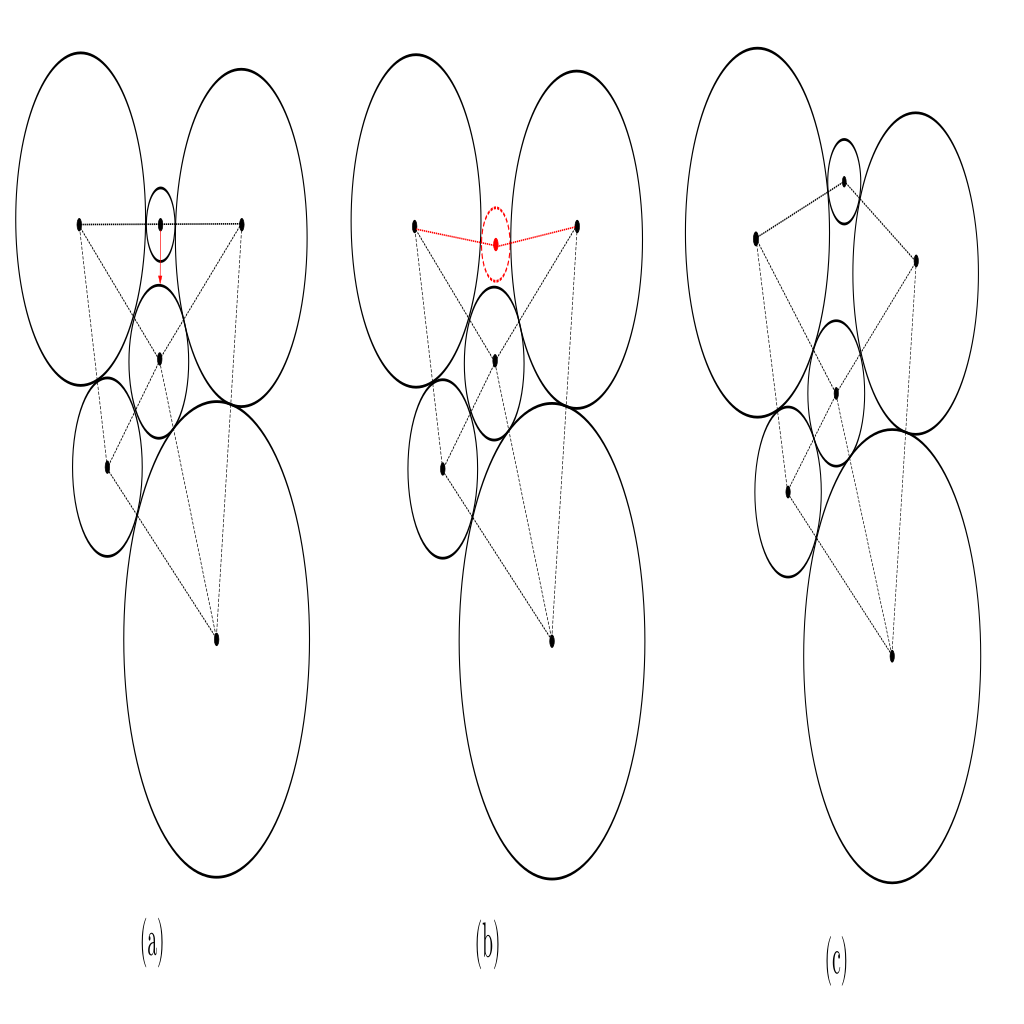
\includegraphics[width = 0.8\textwidth]{Chapter 4/2. Isomorphic but not inf rigid.png}
    \caption{Two isomorphic frameworks. (a) Can be deformed by applying instantaneous velocities (marked in red) on the inner nodes. (b) An infinitesimally rigid framework isomorphic to the one in (a).}
    \label{fig4: iso but not rig}
\end{figure}
\vspace{-3mm}
\begin{flushleft}
We try to unpack this question computationally. By finding known, non-trivial examples for which the conjecture holds, we can contemplate proving the conjecture for general cases. Thus, the two key players here are going to be modules written in Python called \texttt{Rigidity.py} and \texttt{Circle\_Packing.py}. 
\end{flushleft}

\begin{flushleft}
Titled aptly, the module \texttt{Rigidity} takes in a graph and verifies whether it is infinitesimally rigid, and \texttt{Circle\_Packing} takes a planar graph and attempts to find its circle packing using optimization methods. The graphs we'll be analyzing are all Laman graphs on $n \in [3, \hdots, 10]$ vertices.  
\end{flushleft}

\begin{flushleft}
The generation of minimally rigid graphs on $n = 3,4,5$ vertices can be easily done by hand using the Henneberg Constructions from Theorem \ref{def: henneberg}, henceforth abbreviated to $H_1$ and $H_2$ for Type I and Type II respectively. Starting with a Laman graph on 3 vertices (a triangle):
\begin{itemize}
    \item To obtain the Laman graphs on 4 vertices, we can note that applying $H_1$ yields a graph isomorphic to the one we get when applying $H_2$. so there is only one Laman graph on $4$ vertices. 
    \item To obtain the Laman graphs on 5 vertices, we apply $H_1$ to obtain three non-isomorphic graphs with 7 edges. They can be shown to be non-isomorphic by comparing the degrees of each vertex, and the cycle structure within the graph.
\end{itemize}

\noindent
This is illustrated in Figures \ref{fig4: n = 4 Laman} and \ref{fig4: n = 5 Laman}.
\end{flushleft}
\vspace{-4mm}
\begin{figure}[htbp]
    \centering
    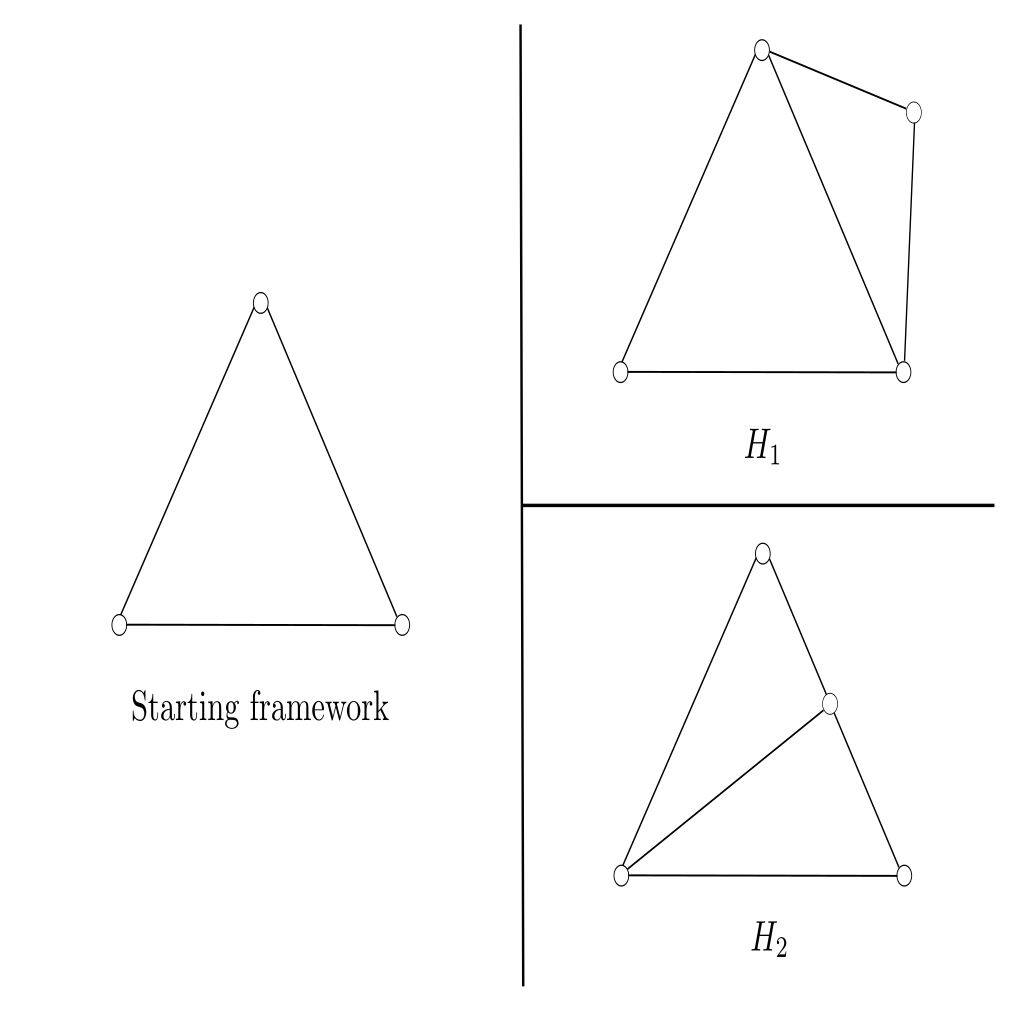
\includegraphics[width = 0.55\textwidth]{Chapter 4/3. n=4.png}
    \caption{Two isomorphic Laman graphs on 4 vertices}
    \label{fig4: n = 4 Laman}
\end{figure}

\begin{figure}[htbp]
    \centering
    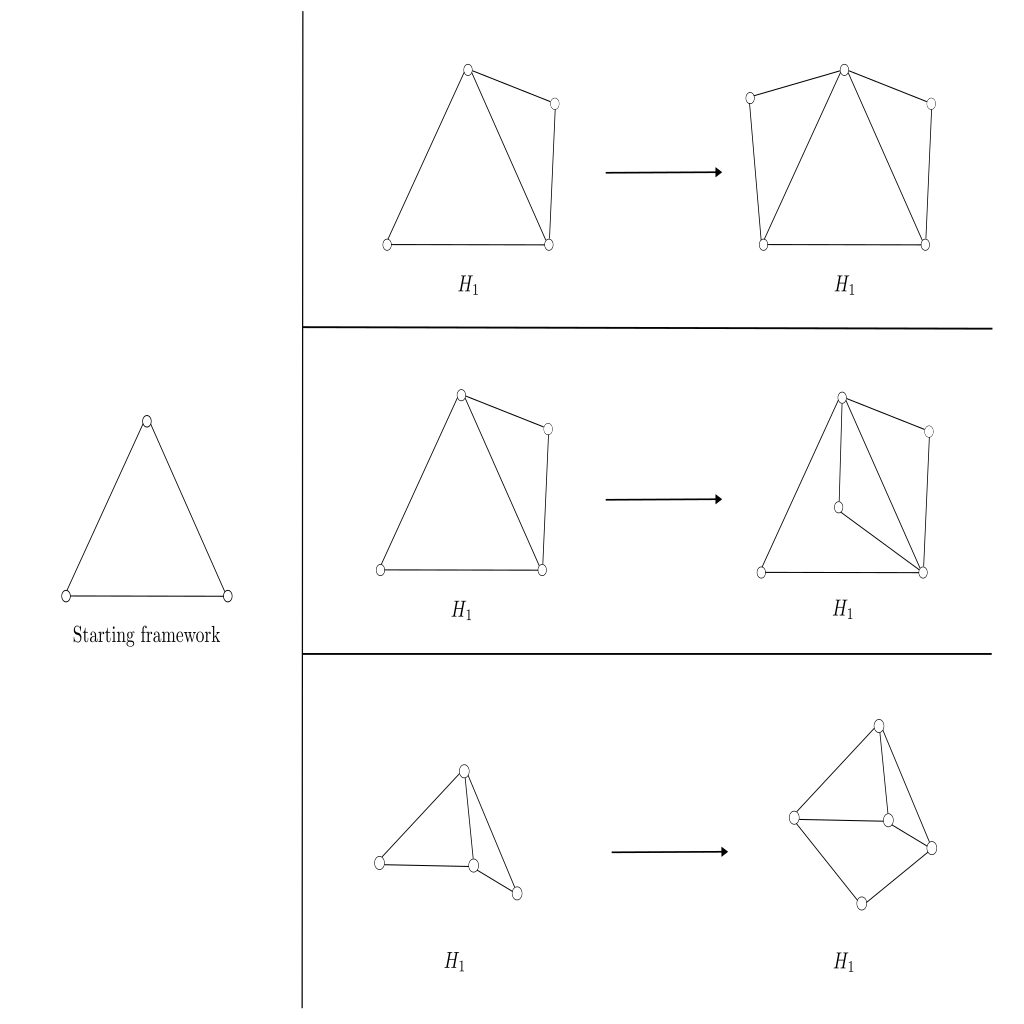
\includegraphics[width = 0.95\textwidth]{Chapter 4/4. n=5.png}
    \caption{The three non-isomorphic Laman graphs on 5 vertices}
    \label{fig4: n = 5 Laman}
\end{figure}

\begin{flushleft}
Planar graphs on vertices $n > 5$ are generated using \texttt{nauty} \cite{nauty}, which allows for the generation of non-isomorphic graphs with a specified number of vertices and edges and saves them as a \texttt{.g6} file. So for example, if we wanted to generate all planar graphs on 8 vertices with 13 edges, we would input
\end{flushleft}

\begin{center}
\texttt{./geng 8 13 | ./planarg | gzip > planar-8-13.g6}    
\end{center}

\begin{flushleft}
into the terminal. This produces a file named \texttt{planar-8-13.g6}, which contains a list of non-isomorphic planar graphs with the required vertices and edges. At this point, we would invoke the two modules \texttt{Rigidity.py} and \texttt{Circle\_Packing.py} to find the minimally rigid graphs and attempt to pack them.     
\end{flushleft}

\begin{flushleft}
    Visually, we can represent what we're trying to do in Figure \ref{fig4: config space}. For a given planar graph $G$ with $n$ vertices and $2n - 3$ edges, there can be a multitude of ways to draw frameworks for it. Referring to Figure \ref{fig4: config space}, we can visualize this as the \textit{space} of frameworks on $G$. Within this space, we have all the frameworks on $G$, some of which are infinitesimally rigid, given as blue lines.  
\end{flushleft}

\begin{figure}[htbp]
    \centering
    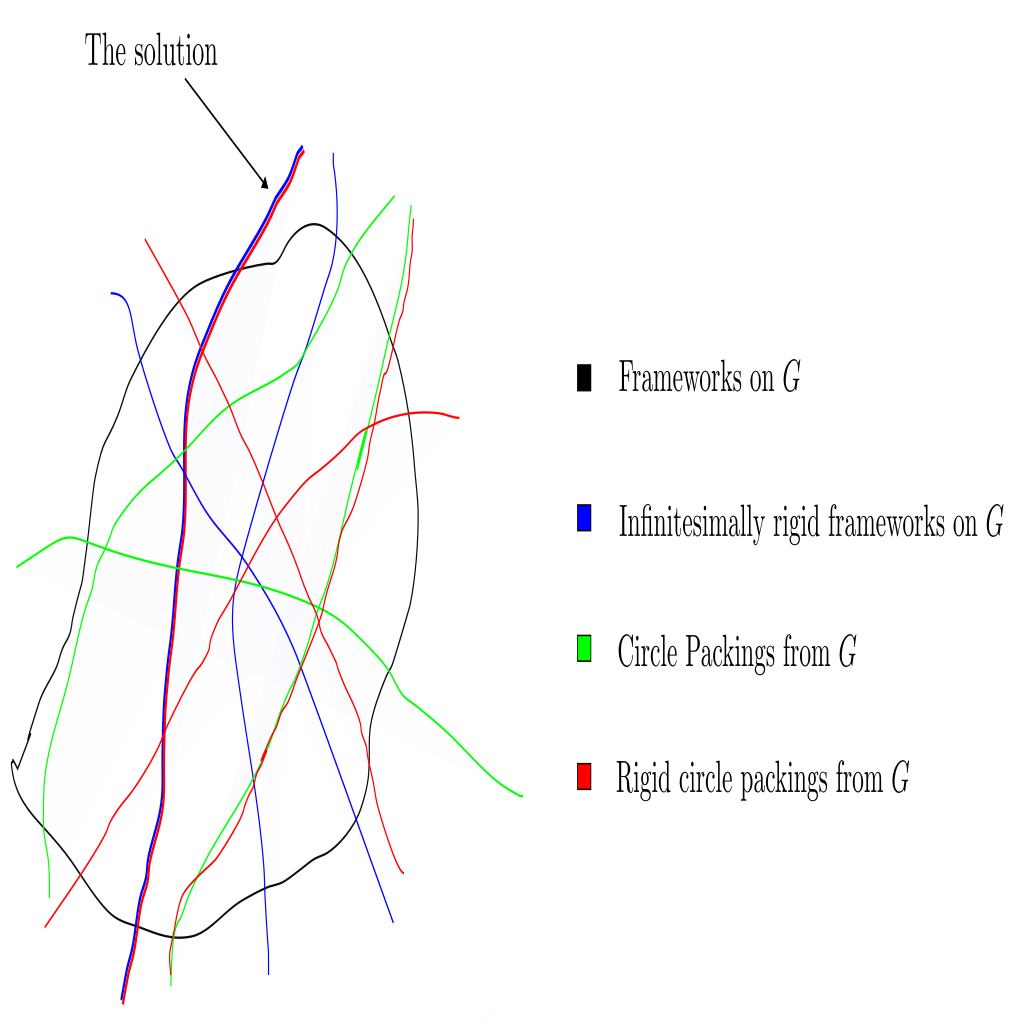
\includegraphics[width = 0.75\textwidth]{Chapter 4/5. configuration space.png}
    \caption{The space containing all frameworks on a graph $G$ drawn as a black outline, the frameworks on $G$ that are infinitesimally rigid drawn as blue lines, the circle packings obtained from $G$ drawn as green lines, and the rigid circle packings obtained from $G$ drawn as red lines.}
    \label{fig4: config space}
\end{figure}
\vspace{-4mm}
\begin{flushleft}
Now, for any circle packing obtained from $G$, its underlying contact graph could either be rigid or not, and so we have green lines to represent any circle packing we can get from $G$. Red lines are used to denote what we are after, the rigid circle packings. 
\end{flushleft}

\begin{flushleft}
Thus, the task is to find where the blue and the red lines overlap! That is, we want to find an infinitesimally rigid planar graph such that it produces a circle packing whose contact graph is also infinitesimally rigid (as this implies rigidity). Such an overlap has been made bold in the Figure. 
\end{flushleft}

\begin{flushleft}
Now that we have an understanding of what it is we're trying to do, let us dive into how we go about doing it! By exploring each module individually, we gain an understanding of what is being done. After that, we can go ahead and use the modules in order to find the packings of interest. All the code described in this chapter can be viewed on Github at \href{https://github.com/Titwik/Dissertation}{Titwik/Dissertation}.
\end{flushleft}

\section{\texttt{Rigidity.py}}

\begin{flushleft}
The first module we visit is the one we will be using to check for the rigidity of a given graph. To do this, we will need to compute the rigidity matrix from Definition \ref{def: rigidity matrix}, and then check whether its rank satisfies Theorem \ref{thm: rank-rigid}. From this point onwards, $n$ shall denote the number of vertices/nodes in a graph/framework, and $m$ shall denote the number of edges in the graph. 
\end{flushleft}

\begin{flushleft}
The graphs we will be considering are constructed using an existing module in Python known as \texttt{networkx} \cite{networkx}, allowing for the study and visualization of graphs in Python. Along with this, to create the rigidity matrix, we use a module called \texttt{numpy} \cite{numpy}. By using built-in structures and functions, such as arrays and functions related to analyzing arrays, we create the rigidity matrix as a \texttt{numpy} array and then use a function to compute its rank.
\end{flushleft}

\begin{flushleft}
This module contains several functions designed to do a particular task, so we visit each of them in turn.
\end{flushleft}

\subsection{Creating a Configuration}

\begin{flushleft}
As touched upon before, a graph is an abstract mathematical object that can be drawn in a multitude of ways. There is no concept of `distance', or the vertices having `coordinates' in $\mathbb{R}^2$. In order to study the rigidity of the graph, we must first take the vertices and give them coordinates, effectively forming a configuration of points. This brings us to the first function in this module, called \texttt{G\_configuration}.
\end{flushleft}

\begin{flushleft}
The function \texttt{G\_configuration} takes in a single argument \texttt{G}, a \texttt{networkx} graph, and begins by learning the number of vertices the graph has. For each vertex then, it randomly assigns an integer for $x$-coordinate and the $y$-coordinate from the interval $[-2^{40}, 2^{40}]$. 
Sampling for coordinates from such a large range of numbers ensures that the points are in a generic configuration, ensuring that we avoid the situation described in Figure \ref{fig: non-generic}. Finally, it returns two lists, one containing the randomly assigned $x$-coordinates and the other containing the randomly assigned $y$-coordinates.
\end{flushleft}

\begin{flushleft}
Now, we have a number of points, each equipped with their own pair of $(x,y)$ coordinates. The next step is to construct the rigidity matrix.
\end{flushleft}

\subsection{Constructing the Rigidity Matrix}

\begin{flushleft}
We define the function \texttt{rigidity\_matrix} which takes in a graph \texttt{G}, and computes its rigidity matrix with the aid of the function \texttt{G\_configuration}. Recalling Definition \ref{def: rigidity matrix}, the rigidity matrix in $\mathbb{R}^2$ has $m$ rows and $2n$ columns. Knowing this, we can initialise a \texttt{numpy} array on $m$ rows and $2n$ columns, and have every entry in the array be 0.
\end{flushleft}

\begin{flushleft}
The task at this stage is to fill in the appropriate entries of the matrix with the correct values. We use the notation $x_i$ and $y_i$ when talking about the $x$-coordinate and the $y$-coordinate of node $i$ respectively. The computation of the entries of the rigidity matrix is done by using the \texttt{enumerate} function, and we keep track of the row index \texttt{i}, as well as the edge \texttt{(u,v)} with each iteration.
\begin{enumerate}
    \item The element in row \texttt{i} and column \texttt{2u} is the $x_u - x_v$.
    \vspace{-3mm}
    \item The element in row \texttt{i} and column \texttt{2u+1} is the $y_u - y_v$.
    \vspace{-3mm}
    \item The element in row \texttt{i} and column \texttt{2v} is the $x_v - x_u$.
    \vspace{-3mm}
    \item The element in row \texttt{i} and column \texttt{2v+1} is the $y_v - y_u$.
\end{enumerate}
The function then returns the rigidity matrix with the modified elements. 
\end{flushleft}

\begin{flushleft}
To test whether this function works as expected, we can try to compute the rigidity matrix of the framework given in Example \ref{eg: rigidity matrix}. This framework has nodes with coordinates $(1,2), (0,0), (2,0)$ and $(1,1)$. 
\end{flushleft}

\begin{flushleft}
By defining the graph \texttt{G} appropriately, and by tweaking the function \texttt{rigidity\_matrix} slightly in order to take the specified coordinates rather than the random ones obtained from \texttt{G\_configuration}, we can compute the rigidity matrix for the example.
\end{flushleft}

\begin{code}
    In: print(rigidity_matrix(G))

    Out: [[ 1.  2. -1. -2.  0.  0.  0.  0.]    # edge (1,2)
          [ 0.  1.  0.  0.  0.  0.  0. -1.]    # edge (1,4)
          [-1.  2.  0.  0.  1. -2.  0.  0.]    # edge (1,3)
          [ 0.  0. -1. -1.  0.  0.  1.  1.]    # edge (2,4)
          [ 0.  0. -2.  0.  2.  0.  0.  0.]]   # edge (2,3)
\end{code}    

\begin{flushleft}
Comparing this to the rigidity matrix computed by hand in Example \ref{eg: rigidity matrix}, we see that while the order of the edges considered has changed, the entries along each corresponding row have not. Thus, we can safely say the function \texttt{rigidity\_matrix} computes the rigidity matrix for a given graph correctly.
\end{flushleft}

\subsection{Rank of the Rigidity Matrix}

\begin{flushleft}
From Theorem \ref{thm: rank-rigid}, we know that the framework is infinitesimally rigid if and only if the rank of the rigidity matrix is equal to $2n-3$. In order to obtain the rank of a matrix in Python, we make use of the \texttt{linalg} library within \texttt{numpy}. 
\end{flushleft}

\begin{flushleft}
To start, we define a function \texttt{check\_rigidity} which takes a graph \texttt{G}, and calls on the \texttt{rigidity\_matrix} function to get the rigidity matrix of \texttt{G}. From here, we use \texttt{np.linalg.matrix\_rank} to compute the rank of the matrix. If the rank is equal to $2n-3$, the function returns \texttt{True}, and \texttt{False} if the condition fails.
\end{flushleft}

\begin{flushleft}
Considering the framework in Example \ref{eg: rigidity matrix}, we know it is infinitesimally rigid by observation as it is a Laman graph on 4 vertices, and this is infinitesimally rigid by Corollary \ref{cor: laman => inf rigid}. By calling this framework \texttt{G}, let us print the rank of the rigidity matrix of \texttt{G}.
\end{flushleft}

\begin{code}
    In: print(np.linalg.matrix_rank(rigidity_matrix(G)))

    Out: 5
\end{code}

\begin{flushleft}
As $(2 \times 4) - 3 = 5$, we confirm that this framework is indeed infinitesimally rigid. Now, to verify whether \texttt{check\_rigidity} works as expected, we print its result using \texttt{G} as the argument. 
\end{flushleft}

\begin{code}
    In: print(check_rigidity(G))

    Out: True
\end{code}

\begin{flushleft}
Thus, we have written a function that now tells us whether a graph is infinitesimally rigid or not.
\end{flushleft}

\subsection{Checking rigidity for a list of graphs}

\begin{flushleft}
By using \texttt{nauty}, we create a list containing all the non-isomorphic planar graphs on a specified number of vertices and edges. Therefore, the last function this module contains is one that filters this list for all the minimally rigid graphs that we want to analyze. In addition to this, we also filter out graphs that have a vertex of degree one or two. 
\end{flushleft}

\begin{flushleft}
If a graph has a vertex with degree one, then it is not rigid and will be discarded when the \texttt{check\_rigidity} function is called. On the other hand, a vertex of degree two can be constructed using a Henneberg Type I construction, and we can pack this vertex by simply creating a circle tangent to two other circles. It is a trivial process and for this reason, such graphs are not very interesting to look at.
\end{flushleft}

\begin{flushleft}
We start defining the function \texttt{find\_rigid\_graphs} by allowing the argument to be a list of graphs. As this list contains graphs, each with the same number of vertices, we choose the first graph in the list and let $n$ be the number of vertices in this graph. 
\end{flushleft}

\begin{flushleft}
In order to filter out the graphs containing a vertex of degree of two, we first loop through all the graphs in the list, and then loop through each vertex in each graph. If the graph does \textbf{not} contain a vertex with degree two, then we add it to a separate list called \texttt{graphs\_without\_degree\_2}. 
\end{flushleft}

\begin{flushleft}
From here, we loop through all the graphs in \texttt{graphs\_without\_degree\_2}, check its rigidity using \texttt{check\_rigidity}, and add it to a new list called \texttt{rigid\_graphs}. Finally, the function \texttt{find\_rigid\_graphs} returns \texttt{rigid\_graphs}, a list containing all planar minimally rigid graphs of minimum degree at least three.
\end{flushleft}

\subsection{Testing the code}

\begin{flushleft}
The last thing to do is to ensure that the code works for known examples before we start investigating graphs we know nothing about. Graphs that are not infinitesimally rigid can be seen in Figures \ref{eg: not_rigid} and \ref{eg: not inf rigid 2.0}. For an additional graph that is known to be infinitesimally rigid, we consider the Framework in Figure \ref{eg: inf rigid}. We label these graphs \texttt{G1}, \texttt{G2} and \texttt{G3} respectively, and construct them using \texttt{networkx}.
\end{flushleft}

\begin{figure}[htbp]
    \centering
    \begin{tabular}{c c c}
        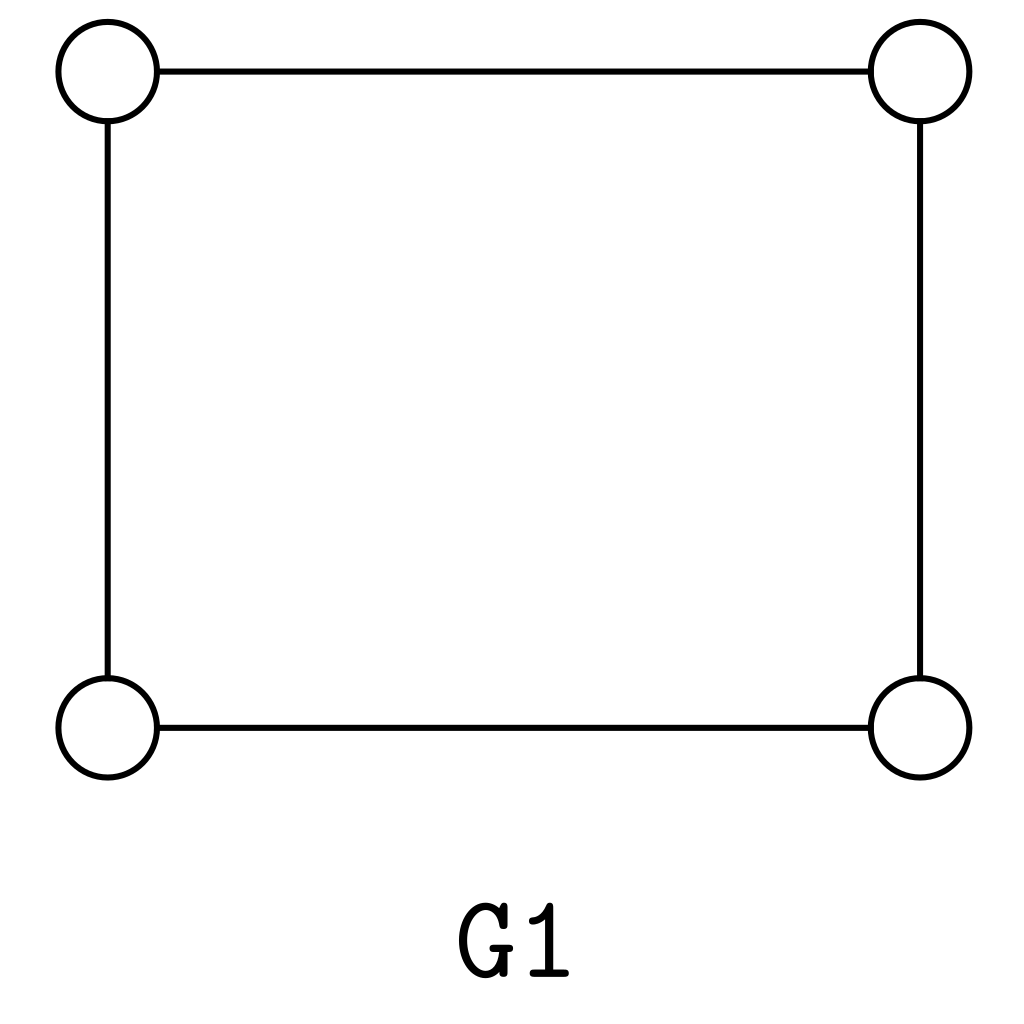
\includegraphics[width = 0.25\textwidth]{Chapter 4/6. not_rigid.png} 
        & 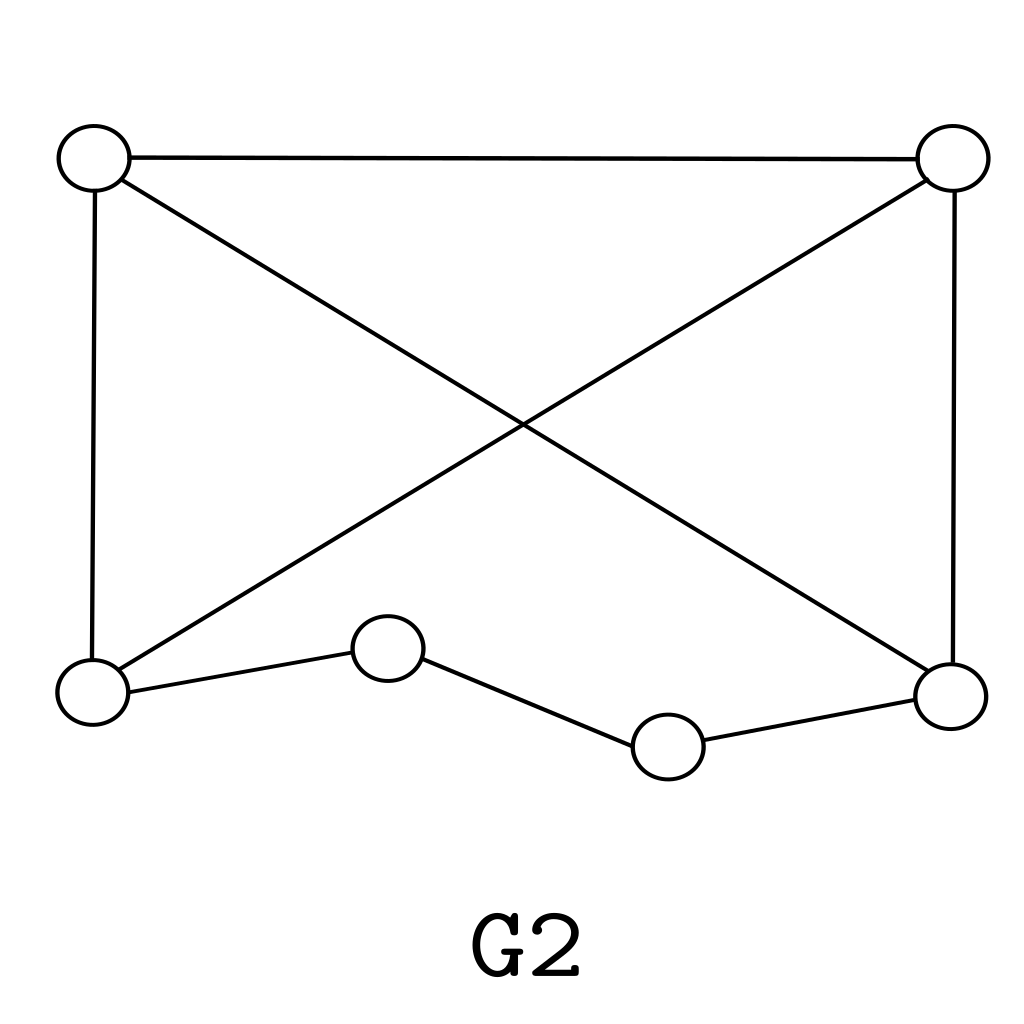
\includegraphics[width = 0.25\textwidth]{Chapter 4/7. not_inf_rigid_2.0.png} &
        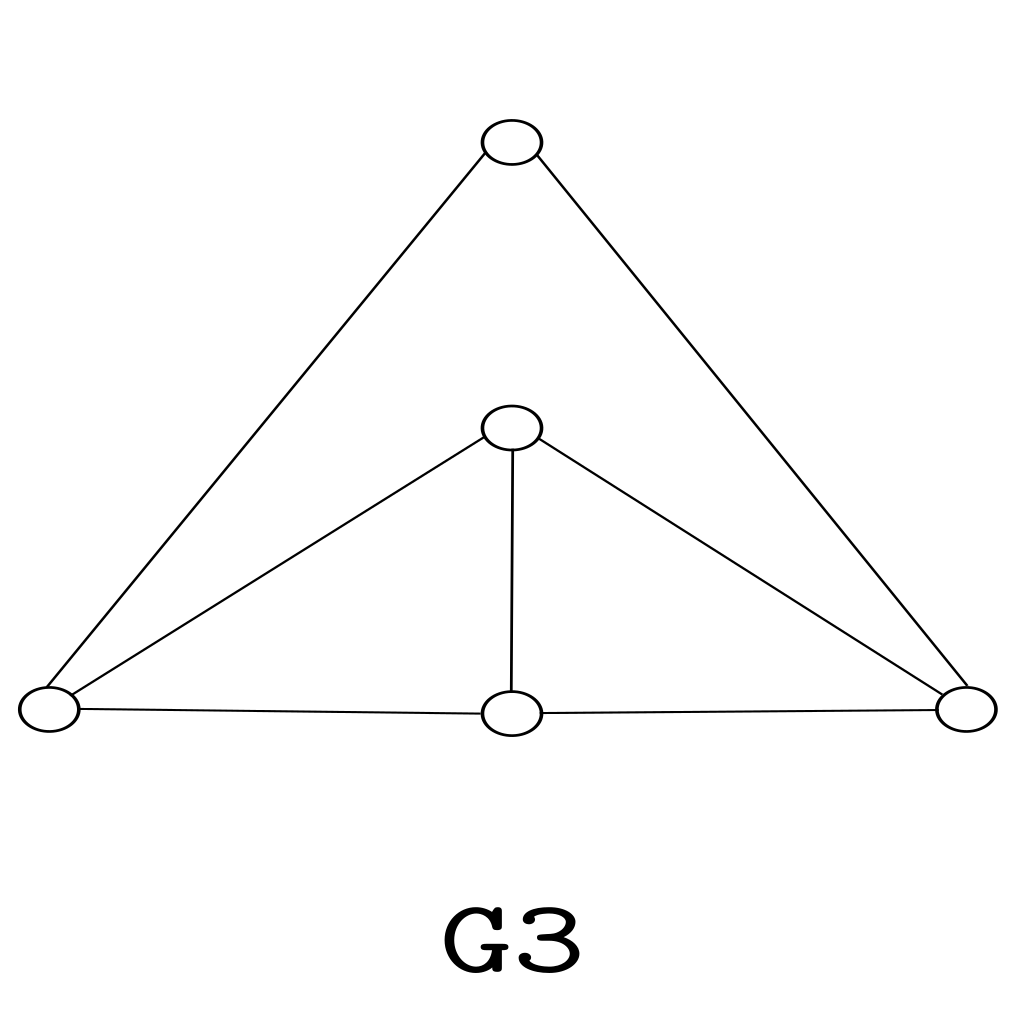
\includegraphics[width=0.2\textwidth]{Chapter 4/8. inf_rigid.png}        
    \end{tabular}
    \caption{The frameworks from Figures \ref{eg: not_rigid}, \ref{eg: not inf rigid 2.0} and \ref{eg: inf rigid} labelled as \texttt{G1}, \texttt{G2}, and \texttt{G3} respectively.}
\end{figure}

\begin{code}
    In [1]: print(check_rigidity(G1))
    Out: False 
    
    In [2]: print(check_rigidity(G2))
    Out: False
    
    In [3]: print(check_rigidity(G3))
    Out: True
\end{code}

\begin{flushleft}
This is reassuring to see! We've successfully verified that the functions work well with each other, and that their outputs are as expected. So, we can confidently identify infinitesimally rigid graphs, and can move onto creating circle packings for a given planar graph. 
\end{flushleft}

\section{\texttt{Circle\_Packing.py}}

\begin{flushleft}
The process of finding circle packings for a graph involves a process called \textit{numerical minimization}. It is a method in which we try to minimize the variables involved in a given problem subject to clearly defined rules or \textit{constraints}. In order to find circle packings, we first have to define the problem carefully through an \textit{objective function}, impose certain constraints, generate a `guess' of what the solution might be, and then feed this information into a minimizer. Let us briefly run through exactly what this module covers. 
\end{flushleft}

\begin{flushleft}
It is made up of four functions, each performing a specific task, similar to how the functions were defined in \texttt{Rigidity.py}. 
\begin{enumerate}
    \item The first of these functions defines the objective function that we want to minimize.
    \vspace{-3mm}
    \item The second function imposes the constraints that the minimization process should obey. 
    \vspace{-3mm}
    \item The third function generates a random list of initial conditions for the coordinates of every node in the framework, as well as randomly generated radii for the circles they inhabit.
    \vspace{-3mm}
    \item The very last function is one that uses the three previous functions in order to generate a circle packing for a graph.
\end{enumerate}
\end{flushleft}

\begin{flushleft}
The minimizer that we will be using comes from the \texttt{scipy} \cite{scipy} library in Python called \texttt{scipy.optimize.minimize}, which we refer to as \texttt{minimize} from now on. To illustrate how this minimizer works, let us do a simple example.
\end{flushleft}

\subsection{Using the Minimizer: A Simple Example}

\begin{flushleft}
Suppose we have a rectangle of length $x$ and width $y$, and we wish to maximize its area $xy$, subject to the constraint that its perimeter is 20 units. Translating this into something that we can use in the minimizer, the objective function would be $-xy$ as we are trying to maximize the area with the minimize function. The constraint can be modelled as $2x+2y = 20$ and our initial guesses for the values of $x$ and $y$ could be 6 and 4 respectively. 
\end{flushleft}

\begin{flushleft}
We would input this into the \texttt{minimize} function, and obtain the optimal values of $x$ and $y$ satisfying these constraints such that the area of the rectangle is maximized. The code for this example is shown below.
\end{flushleft} 

\begin{code}
    # define the objective function
    def area_rectangle(xy):
        x = xy[0]
        y = xy[1]
        area = xy[0] * xy[1]
        return -area
    
    # define the constraint
    cons = ({`type':`eq', `fun': lambda xy: 2*xy[0] + 2*xy[1] - 20})
    
    # define the initial condition, where 6 is our initial x value and 
    # 4 is our initial y value
    initial_guess = [6,4]
    
    # use the minimizer
    result = scipy.optimize.minimize(area_rectangle, initial_guess, constraints = cons)
\end{code}

\begin{code}
    In: print(f"x = {result.x[0]} and y = {result.x[1]}")
    Out: x = 5.0 and y = 5.0    
\end{code}

\begin{flushleft}
Therefore, the values of $x$ and $y$ that maximize the area of a rectangle with a perimeter of 20 units are 5 and 5 respectively. Hopefully this example provides some insight into how we can leverage the minimizer. We will not be delving too deep into how the \texttt{minimize} works at this stage, but understanding how to use it properly is imperative for when we attempt to find a circle packing for a graph.
\end{flushleft}

\begin{flushleft}
With that in mind, let us dive into the first function in the \texttt{Circle\_Packing.py} module!
\end{flushleft}

\subsection{Creating the Objective Function}

\begin{flushleft}
Let $(G, \mathbf{p})$ be a framework, $x_i$ and $y_i$ be the $x$-coordinate and $y$-coordinate of node $i$, and $r_i$ be the radius of the circle this node inhabits. We consider the node to be the center of this circle.
\end{flushleft}

\subsubsection{Defining the objective function}

\begin{flushleft}
To begin constructing the function that we wish to minimize, we first consider the distance between two nodes and set it equal to the sum of the radii of the circles they inhabit. That is;

\begin{equation*}
    (x_i - x_j)^2 + (y_i-y_j)^2 = (r_i + r_j)^2 \hspace{16mm} \forall i,j \in V(G)    
\end{equation*}

\vspace{2mm}
When using the minimizer however, we must input this equation such that the right hand side must be equal to 0. Therefore, we write this as 

\begin{equation*}
    (x_i - x_j)^2 + (y_i-y_j)^2 - (r_i + r_j)^2 = 0 \hspace{10mm} \forall i,j \in V(G)
\end{equation*}

\vspace{2mm}
As we saw in the example above, by trying to minimize a negative objective function, we end up maximizing it instead. To avoid such complications arising in this scenario, we square the entire function so that the values we work with are strictly positive.

\begin{equation*}
    ((x_i - x_j)^2 + (y_i-y_j)^2 - (r_i + r_j)^2)^2 = 0 \hspace{11mm} \forall i,j \in V(G)
\end{equation*}

\vspace{2mm}
At this stage, we will have several equations, one for each pair of nodes. The final step to obtain the objective function will be to consider the sum of all these equations. Therefore, the function that we treat as our objective function will be 

\begin{equation}\label{eq:circle_constraint}
    \sum_{\substack{i,j=1 \\ i \neq j}}^{n} \left( (x_i - x_j)^2 + (y_i - y_j)^2 - (r_i + r_j)^2 \right)^2
  \end{equation}
\end{flushleft}

\subsubsection{Writing the code}

\begin{flushleft}
To input Equation \ref{eq:circle_constraint} as the objective function into the minimizer, we first define a function \texttt{mk\_obj} that takes in a graph \texttt{G}, and construct another function named \texttt{objective\_function} within this function like so;
\end{flushleft}

\begin{code}
    # function that returns the objective function
    def mk_obj(G):
        
        # create a function that computes the objective function of a graph G
        def objective_function(vars):
        ...
\end{code}

\begin{flushleft}
The argument \texttt{vars} represents a list of the variables \texttt{[x1,y1,r1, ... , xn,yn,rn]}. These are the variables that will be minimized when we use the minimizer, where \texttt{xi} and \texttt{yi} represent the $x$-coordinate and $y$-coordinate respectively of node $i$, and \texttt{ri} is the radius of the circle this node centers.
\end{flushleft}

\begin{flushleft}
Inside \texttt{objective\_function}, we define three new functions, \texttt{x(i)}, \texttt{y(i)} and \texttt{r(i)}:

\begin{enumerate}
    \item The function \texttt{x(i)} returns \texttt{vars[3*i]}.
    \vspace{-3mm}
    \item The function \texttt{y(i)} returns \texttt{vars[3*i+1]}.
    \vspace{-3mm}
    \item The function \texttt{r(i)} returns \texttt{vars[3*i+2]}.
\end{enumerate}

For example, the $x$-coordinate of every node occurs in positions 0, 3, 6, ..., in \texttt{vars}, and so the function \texttt{x(i)} returns every third element of \texttt{vars}. The remaining two functions are definined similarly.
\end{flushleft}

\begin{flushleft}
Lastly, we initialise a variable \texttt{total} to store the sum of the objective functions, and set it to 0. Looping through all the edges $(i,j) \in E(G)$, we compute the sum given in Equation \ref{eq:circle_constraint}, and return this sum as follows;
\end{flushleft}

\begin{code}
    # initialise a sum
    total = 0
    
    # compute the sum 
    for (i,j) in G.edges():
        total += ((x(i) - x(j)) ** 2 + (y(i) - y(j)) ** 2 - (r(i) + r(j)) ** 2) ** 2
    
    # return the sum
    return total
\end{code}

\begin{flushleft}
All that's left to do is to return the output of the \texttt{objective\_function} as the output of \texttt{mk\_obj}.
\end{flushleft}

\begin{code}
    def mk_obj(G):
        def objective_function(vars):
            ...
            return total
        return objective_function
\end{code}

\begin{flushleft}
This completes the function \texttt{mk\_obj}, a function that takes in a graph, and returns its objective function. By feeding this into the minimizer, we are essentially telling the computer to make each variable in the list \texttt{vars} as small as they can be. The next step we will need to take is informing the minimizer of the constraints that should be obeyed.
\end{flushleft}

\subsection{Defining the Constraints}

\begin{flushleft}
The constraints can be thought of rules that the minimizer must follow. In our case, to generate a circle packing such as the one in Figure \ref{fig: circle packing example}, the constraints we impose are:

\begin{enumerate}
    \item Each circle must have a positive radius.
    \vspace{-3mm}
    \item Each circle must have a maximum radius.
    \vspace{-3mm}
    \item The circles must not overlap or contain each other.
\end{enumerate}

To present these constraints to the minimizer, we code each one carefully, add it to a list named \texttt{constraints}, and then feed this list to the minimizer. By adhering to these rules, the minimizer will produce a configuration of circles, each equipped with a radius, such that the conditions required for a circle packing are satisfied. We begin by creating a function \texttt{cons}, which takes a graph \texttt{G} as its argument, and tackle each constraint mentioned in the list above individually.
\end{flushleft}

\subsubsection{1. Each circle must have a positive radius.}

\begin{flushleft}
To ensure that the radius is positive, we set a tolerance value \texttt{epsilon} such that the radius must be at least \texttt{epsilon}. Setting this tolerance as 0 is not possible as it leads to a host of problems due to the nature of floating point arithmetic (which we will not discuss any further). 
\end{flushleft}

\begin{flushleft}
Choosing an appropriate tolerance can be challenging as if it were too big, then we disallow circles of very small radii to be formed, which may not converge to a circle packing. On the other hand, picking a value too small can lead to numerical instability due to the nature of optimization, as well as increase the time it takes for the minimizer to converge to a solution.
\end{flushleft}

\begin{flushleft}
After some trial and error, letting \texttt{epsilon = 0.04} strikes the balance of achieving accurate circle packings in a reasonable duration of time. To enter the constraint in a format the minimizer will accept, we first loop through every vertex in \texttt{G}, indexed by \texttt{i}, and write the constraint as 
\end{flushleft}

\begin{code}
    # radius must be greater than epsilon constraint
    {`type': `ineq', `fun': lambda vars, i=i: vars[3*i + 2] - epsilon}
\end{code}

\begin{flushleft}
Let us consider each term in this entry individually:

\begin{itemize}
    \item (\texttt{`type': `ineq'}) means that the constraint that we are entering is an inequality.
    \vspace{-3mm}
    \item (\texttt{`fun': lambda vars, i=i}) means that the function we are using is one named \texttt{lambda}, and this function takes in arguments \texttt{vars} and \texttt{i}.
    \vspace{-3mm}
    \item (\texttt{vars[3*i + 2] - epsilon}) is the inequality $r_i > \epsilon$ that we use to define positive radii. As the right hand side must be 0, we consider the inequality $r_i - \epsilon > 0$.
\end{itemize}

We then add this to the list \texttt{constraints}, and move onto the next constraint we wish to impose. 
\end{flushleft}

\subsubsection{2. Each circle must have a maximum radius.}

\begin{flushleft}
We set a maximum radius to ensure computational efficiency, and also prevent the creation of excessively large circles that could obscure the other circles present in the packing. This guarantees that all circles are visible and the arrangement remains visually appealing. 
\end{flushleft}

\begin{flushleft}
Here, the maximum radius chosen will be 10 units, and is implemented as a constraint by looping through every vertex in \texttt{G}, indexed by \texttt{i}. Adding
\end{flushleft}

\begin{code}
    {`type': `ineq', `fun': lambda vars, i=i: 10 - vars[3*i + 2]}
\end{code}

\begin{flushleft}
to the list \texttt{constraints}, we continue to write the final constraint we need to implement.
\end{flushleft}

\subsubsection{3. The circles must not overlap or contain each other.}

\begin{flushleft}
By implementing the two constraints above, we have guaranteed the existence of circles in our packing. However, there is nothing stopping a circle from extending over into another circle's interior. This also includes the scenario where one circle lies completely within another circle. From Definition \ref{def: circle packing}, we know that each circle must either be tangential with another, or have nothing to do with each other.
\end{flushleft}

\begin{flushleft}
In order to achieve this, we set a final constraint such that the distance between any two nodes in $G$ must be at least the sum of the radii of the circles they center. This can be written as

\[
(x_i - x_j)^2 + (y_i - y_j)^2 \geq (r_i + r_j)^2
\]

\vspace{2mm}
for all $i,j \in V(G)$ such that $i \neq j$. Then when we have equality, the circles with centers $(x_i, y_i)$ and $(x_j, y_j)$ are tangential. Otherwise, the circles do not interact.
\end{flushleft}

\begin{flushleft}
We do this by first looping through all the vertices in \texttt{G}, indexed by \texttt{i}, and nesting another loop through the vertices of \texttt{G}, this time indexed by \texttt{j}. As we only want to consider pairs of vertices $(i,j)$ where $i \neq j$, we set an \texttt{if} condition to achieve this. Thus, we add this constraint to our list \texttt{constraints} as;
\end{flushleft}

\begin{code}
    {`type': `ineq', `fun': lambda vars, i=i, j=j: 
    (vars[3*i] - vars[3*j])**2 + (vars[3*i + 1] - vars[3*j + 1])**2 - 
    (vars[3*i + 2] + vars[3*j + 2])**2}
\end{code}

\begin{flushleft}
which allows us to secure a packing where the circles are tangential and their interiors are disjoint! The \texttt{cons} function now returns the list \texttt{constraints} containing the three rules we want our packing to obey. 
\end{flushleft}

\begin{flushleft}
So far, we have our objective function and a list of constraints that the circle packing should stick to. The very last thing that we need before we can invoke the minimizer is a list of initial conditions for the coordinates of each node in the graph, as well as for each radius in the circle packing.
\end{flushleft}

\subsection{Generating Initial Conditions}

\begin{flushleft}
The initial conditions will be generated using a function we define as \texttt{initial\_conditions}, which takes a graph \texttt{G} as an argument. To do this, we make use of the \texttt{random} \cite{random} module in Python. By using a random configuration each time the \texttt{initial\_conditions} function is called, we ensure that the minimizer gets a new place to start from. Doing it this way bypasses the situation where we get stuck trying to pack a configuration known to fail repeatedly.
\end{flushleft}

\begin{flushleft}
We allow the initial $x$ and $y$ coordinates to be obtained from the continuous range $[0,10]$, and the radius $r$ will have initial radii generated from the range $[0,1]$. By choosing a small interval for the initial coordinates of each node, if the initial configuration of points closely matches a circle packing, then we can expect the minimizer to arrive there quickly.
\end{flushleft}

\begin{flushleft}
To start generating the coordinates and radii, we begin by creating a list \texttt{IC}, and then loop through all the nodes in \texttt{G}. For each node, we generate an $x$ and $y$ coordinate using the function \texttt{random.uniform(0,10)} to draw a random number between 0 and 10 uniformly. For each radius $r$, we use \texttt{random.uniform(0,1)} to draw a random number between 0 and 1 uniformly.
\end{flushleft}

\begin{flushleft}
We insert each randomly generated number into \texttt{IC} in the order [$x,y,r$], to match with the variable \texttt{vars} from before. The function \texttt{initial\_variables} finally returns \texttt{IC}, a list containing $n$ initial $x$-coordinates, $n$ initial $y$-coordinates, and $n$ initial radii, totalling $3n$ elements in the list.
\end{flushleft}

\begin{flushleft}
Summarizing everything we have so far, for a given graph \texttt{G}, we have defined functions that take in \texttt{G} and return the objective function that is to be minimized, a list of constraints to adhere to in order to form a circle packing, and a list of initial conditions for the coordinates of each circle's center, as well as their radii. The last step to take is to use the minimizer in order to obtain the circle packing for a planar graph.
\end{flushleft}

\begin{flushleft}
Before we do this though, let's take a quick detour and go through some fundamental ideas of numerical optimization, the issues that arise during minimization, and what we can do to overcome these issues. 
\end{flushleft}

\subsection{Detour: Understanding Optimization}

\begin{flushleft}
The aim of this section is to learn a little bit about what happens behind the scenes when we use the \texttt{minimize} function. In particular, how the initial conditions chosen play a big role in the convergence to a solution. As an example, let us go through how the initial conditions affect the root-finding abilities of the Newton-Raphson method.
\end{flushleft}

\subsubsection{Example: Newton-Raphson Method}

\begin{flushleft}
The Newton-Raphson method is an algorithm used to find the roots $x_r$ of a given function $f(x)$. It is used as follows:
\begin{enumerate}
    \item Pick an initial $x = x_0$, and compute its corresponding $f(x_0)$.
    \vspace{-3mm}
    \item Draw the tangent of $f(x)$ at the point $x = x_0$, and mark the tangent's intersection with the $x$-axis as $x_1$.
    \vspace{-3mm}
    \item Repeat steps 1 and 2 by setting $x_0 = x_1$ until the algorithm converges to $x_r$.
\end{enumerate}

This is shown in Figure \ref{fig: newton}. Clearly, with an increasing number of iterations, our values for $x = x_i$ converge towards the root $x_r$. However, this is dependent on the function $f(x)$, as well as the initial position $x=x_0$ chosen, see Figure \ref{fig: bad newton}. 
\end{flushleft}

\begin{figure}[htbp]
    \centering
    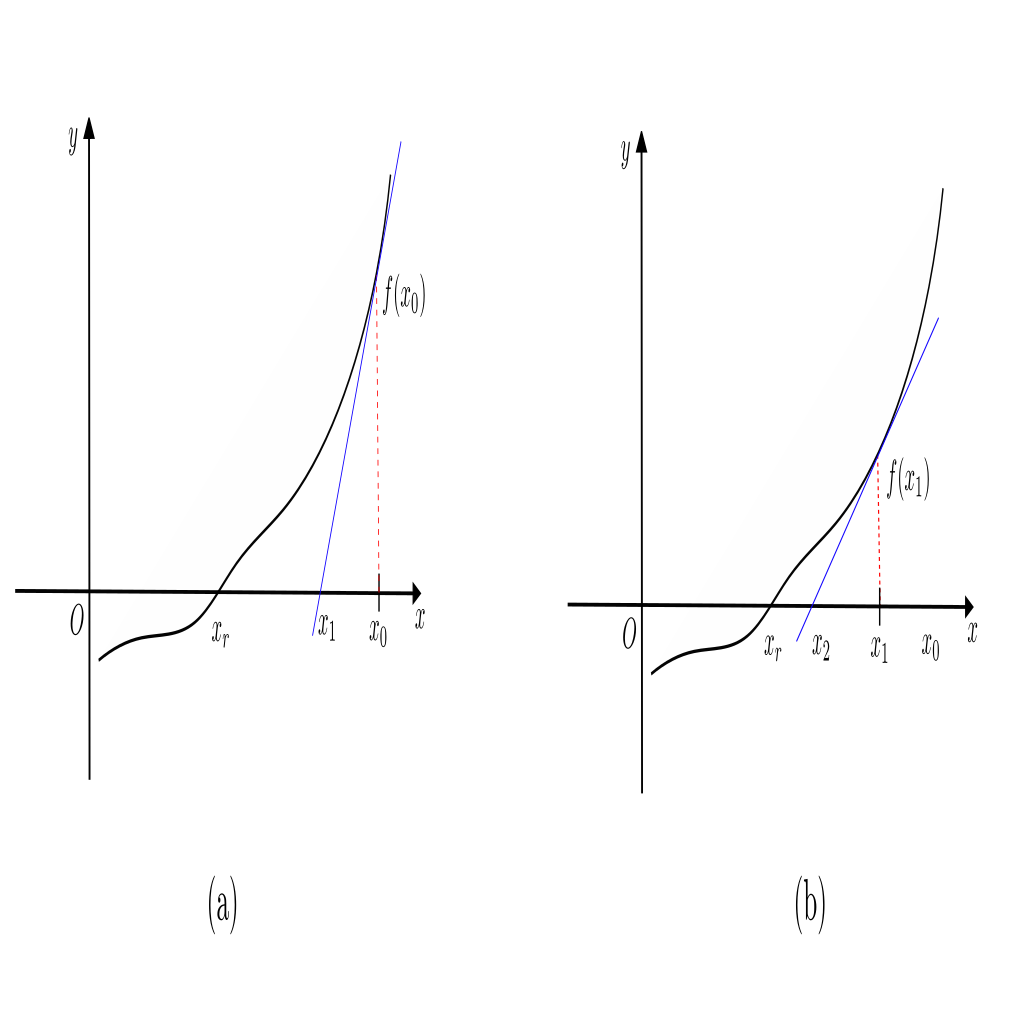
\includegraphics[width = 1\textwidth]{Chapter 4/9. newton raphson.png}
    \caption{(a) First iteration of the Newton-Raphson Method. (b) Second iteration of the Newton-Raphson Method.}
    \label{fig: newton}
\end{figure}

\begin{figure}[htbp]
    \centering
    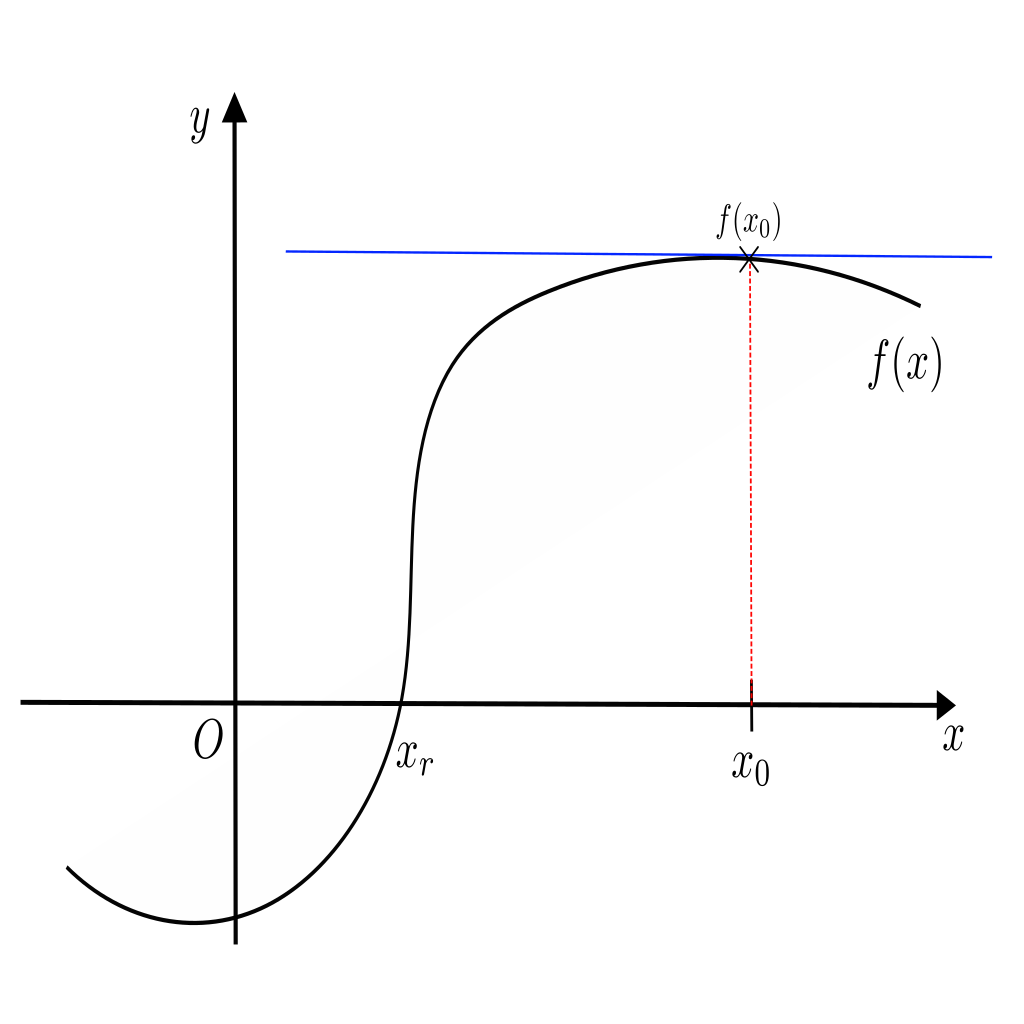
\includegraphics[width = 0.5\textwidth]{Chapter 4/10. bad newton raphson.png}
    \caption{A poorly chosen initial $x=x_0$. The tangent (blue line) will not intersect the $x$-axis anywhere near the root $x_r$.}
    \label{fig: bad newton}
\end{figure}

\vspace{-4mm}
\begin{flushleft}
These two examples showcase how the convergence to a solution can be extremely sensitive to the initial conditions chosen. Choose well, and we converge to the solution ($x_r$ in this case) quickly, but if our initial condition is chosen poorly, the convergence may be significantly delayed or may not occur at all.
\end{flushleft}

\subsubsection{Global vs Local Minimum}

\begin{flushleft}
An additional factor that can prevent us from obtaining a correct circle packing is when the minimizer reaches a \textit{local} minimum, and not the \textit{global} minimum. A circle packing is achieved if only if the minimizer converges to the global minimum. 
\end{flushleft}

\begin{figure}[htbp]
    \centering
    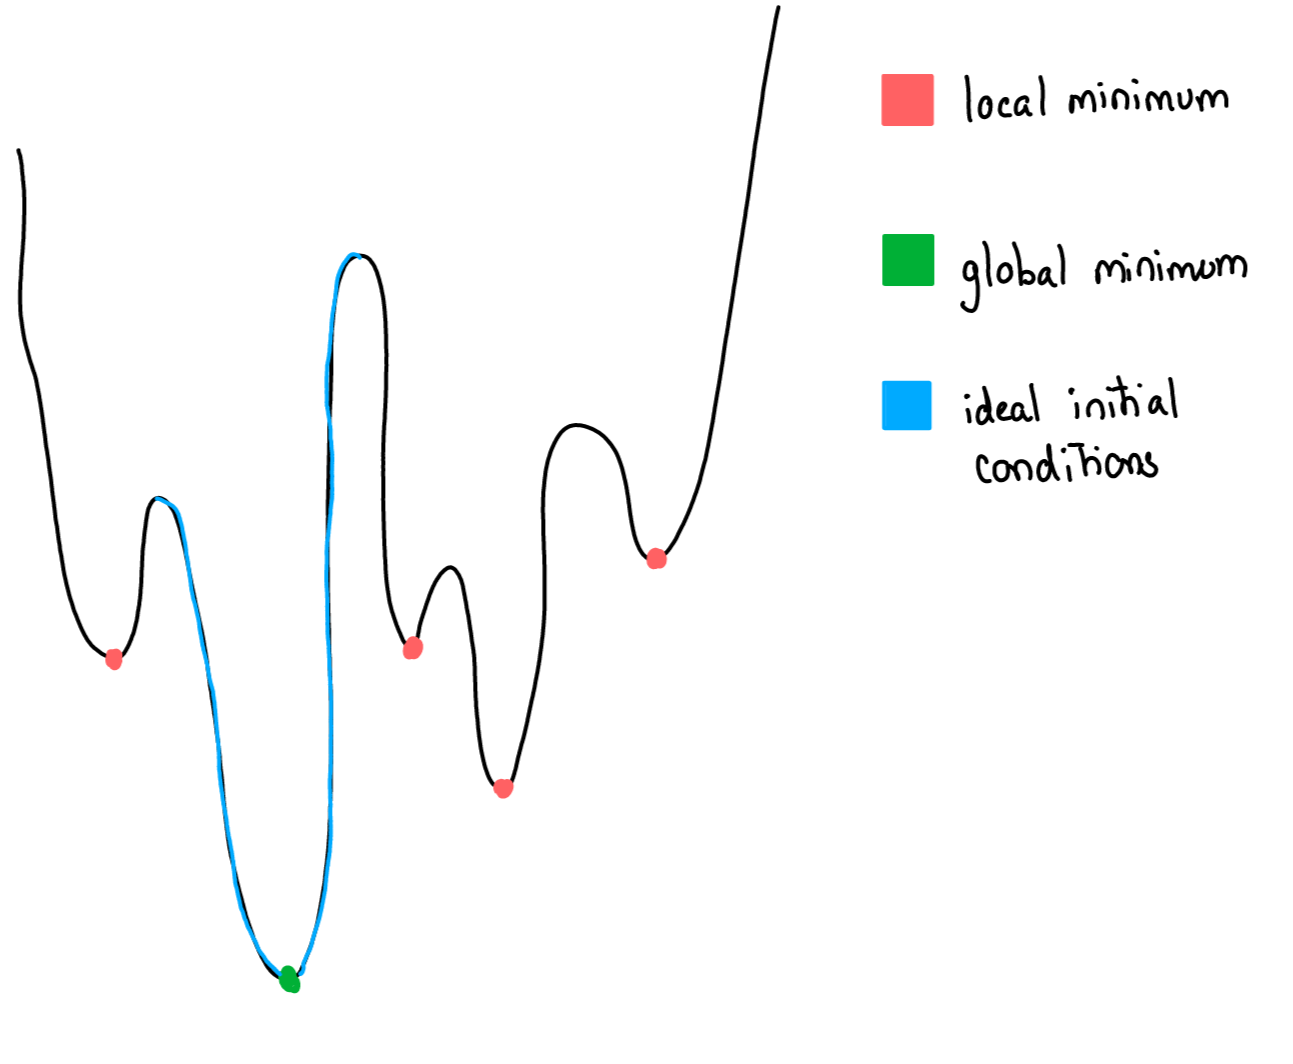
\includegraphics[width = 0.5\textwidth]{Chapter 4/11. energy.png}
    \caption{A visualization of the local minimums and the global minimum the minimizer can achieve. To achieve the global minimum, the initial condition must be along the slopes leading down to the global minimum.}
    \label{fig4: minimum}
\end{figure}

\vspace{-4mm}
\begin{flushleft}
Initial conditions play a part in achieving a global minimum as well. Consider Figure \ref{fig4: minimum}, and suppose we have an initial condition that is placed on one of the slopes descending towards a local minimum (given as red dots). 
\end{flushleft}

\begin{flushleft}
If the minimizer were to start here, then it would minimize the objective function until it reaches a local minimum, believe that it has reached the global minimum, and then return a false solution. Therefore, the ideal initial condition must be on the the slope going down to the global minimum (given as blue slopes).
\end{flushleft}

\subsubsection{Overcoming pitfalls}

\begin{flushleft}
Such a situation can be tricky to navigate. Are we always able to pick suitable initial conditions such that the minimizer attains the global minimum? Moreover, how do we verify that it is indeed at a global minimum? Such questions can be hard to answer in general, but thankfully in our case, we can use some of the tools picked up along the way to aid us!
\end{flushleft}

\begin{flushleft}
The first thing we do is verify whether the minimizer hits a global or local minimum. We know that a correct circle packing is generated when the minimizer achieves a global minimum. Additionally, we know from Definition \ref{def: contact graph} that since our graph $G$ has $2n-3$ edges, the circle packing obtained must also have $2n-3$ contacts. 
\end{flushleft}

\begin{flushleft}
Therefore, we can verify that the minimizer attains a global minimum if and only if the resulting circle packing has $2n-3$ contacts! 
\end{flushleft}

\begin{flushleft}
If the minimizer produces a circle packing that doesn't have $2n-3$ contacts, then this means the initial conditions were unfavorable and it converged to a local minimum. In this case, we call the function \texttt{initial\_conditions}, generating a new random configuration of points and radii, and attempt to pack the graph once more. 
\end{flushleft}

\begin{flushleft}
Armed with the knowledge to combat situations in which the minimizer arrives to an incorrect solution, we embark on the final stretch to complete this module. 
\end{flushleft}

\subsection{Finding Circle Packings}

\subsubsection{Using the minimizer}

\begin{flushleft}
We begin the search for a circle packing of a given graph \texttt{G} by first defining a function \texttt{circle\_packing}, which takes \texttt{G} as an argrument. From here, start a \texttt{while} loop and call the \texttt{minimize} function like so;
\end{flushleft}

\begin{code}
    result = minimize(mk_obj(G), initial_conditions(G), 
                        constraints = cons(G), method='COBYLA')
\end{code}

\begin{flushleft}
where the first argument is the objective function of \texttt{G} we minimize, the second is the list of initial conditions for the configuration of nodes and radii, the third is the list of constraints imposed, and the last argument defines the method of optimization used (Constrained Optimization BY Linear Approximations, or COBYLA)\footnote{should i explain why this method? doesnt seem important}. 
\end{flushleft}

\begin{flushleft}
The list \texttt{result.x} contains all the minimized variables, and recalling how the variable \texttt{vars} was defined in the \texttt{mk\_obj} function, we know that they are stored in the order \texttt{[x1,y1,r1, ..., xn,yn,rn]}. After the \texttt{minimize} function achieves a minimum, we retrieve the $x$ and $y$ coordinates along with the radii $r$ by creating three new lists named \texttt{x\_list}, \texttt{y\_list}, \texttt{r\_list}, looping through \texttt{result.x}, and sorting each element into one of the three lists. 
\end{flushleft}

\begin{flushleft}
For example, the $x$-coordinates are saved in \texttt{x\_list} by;
\end{flushleft}

\begin{code}
    x_list = []

    for i in range(n):
        x = result.x[3*i]
        x_list.append(x)
\end{code}

\subsubsection{Testing for a global minimum}

\begin{flushleft}
Before we use these variables to display a circle packing, we need to make sure that the minimizer achieved a global minimum and not a local one, which happens if the circle packing contains $2n-3$ contacts. We verify this by looping through every pair of coordinates $(x_i,y_i)$, where $x_i$ and $y_i$ are the $x$ and $y$ coordinates of node $i$ respectively, and check whether the the distance between two nodes equals the sum of the radii of their respective circles. We expect $2n-3$ such equalities.
\end{flushleft}

\begin{flushleft}
Initializing a \texttt{counter} with initial value 0, and a \texttt{tolerance} for 0 as 0.001, we check the number of contacts by;
\end{flushleft}

\begin{code}
    for i in range(n):
            x1 = x_list[i]
            y1 = y_list[i]

            for j in range(i+1,n):
                x2 = x_list[j]
                y2 = y_list[j]

                # check if the distance between the centers is equal to the sum of radii
                if abs(np.sqrt((x1 - x2) ** 2 + (y1 - y2) ** 2) - 
                            (r_list[i] + r_list[j])) < tolerance:
                    counter += 1  # add one to the counter
\end{code}

\begin{flushleft}
We continue the code under the \texttt{if counter == (2*n - 3)} condition, as we have a successful packing if this is satisfied. If this condition fails, the loop restarts and the \texttt{minimize} function is called again with a new configuration of points and radii. 
\end{flushleft}

\subsubsection{Creating the contact graph}

\begin{flushleft}
In preparation for the analysis of the circle packings generated, we generate the contact graph of the successful packing as a \texttt{networkx} graph. This done in a very similar fashion to how we checked for $2n-3$ contacts.
\end{flushleft}

\begin{flushleft}
We start by initializing an empty \texttt{networkx} graph called \texttt{contact\_graph}, and if circles centered by nodes $i$ and $j$ are tangential, then we add an edge between nodes $i$ and $j$ in the contact graph. Doing this for every node in the circle packing produces the contact graph of the packing, which will be used later on.
\end{flushleft}

\subsubsection{Generating the circle packing}

\begin{flushleft}
Here, we will be generating three different figures named \texttt{fig1}, \texttt{fig2} and \texttt{fig3}. 
\begin{itemize}
    \item \texttt{fig1} will be the circle packing.
    \vspace{-3mm}
    \item \texttt{fig2} will be the circle packing with its contact graph visualized within the packing.
    \vspace{-3mm}
    \item \texttt{fig3} will be the contact graph of the circle packing. 
\end{itemize}

Let's begin drawing circles!\footnote{do i need the details on how i plotted and scaled the circle packing?}
\end{flushleft}

\begin{flushleft}
We initialize \texttt{fig1}, along with its axis \texttt{ax1} using \texttt{fig1, ax1 = plt.subplots()}. From here, we start a loop over \texttt{n}, the number of nodes in the graph \texttt{G}, and index this loop using \texttt{i}. Recall that the coordinates of the circles in the packing are stored in lists \texttt{x\_list} and \texttt{y\_list}, while the radii are stored in \texttt{r\_list}. We set the variables \texttt{x,y} and \texttt{r} as \texttt{x\_list[i], y\_list[i]}, and  \texttt{r\_list[i]} respectively. Using the \texttt{circle} function from the \texttt{matplotlib} library, we plot the circle with center \texttt{(x,y)} and radius \texttt{r} in \texttt{fig1}. Doing this for every set of coordinates and radii completes the circle packing in \texttt{fig1}.
\end{flushleft} 

\begin{flushleft}
For \texttt{fig2}, we repeat the process done in \texttt{fig1} to plot the same circle packing, with the additions of a visible center and a dashed line between the centers of tangential circles. Finally, \texttt{fig3} drops the plotting of the circles but keeps the plot of the contact graph generated within the packing, as done in \texttt{fig2}.
\end{flushleft}

\begin{flushleft}
At the very end, the function \texttt{circle\_packing} returns the original graph \texttt{G}, the \texttt{networkx} contact graph of the packing \texttt{contact\_graph}, and the figures \texttt{fig1}, \texttt{fig2} and \texttt{fig3}. This completes the module \texttt{Circle\_Packing.py}!
\end{flushleft}

\subsubsection{Testing the code}

\begin{flushleft}
As with the \texttt{Rigidity.py} module, we must test the function \texttt{circle\_packing} on known examples before we venture out into the unknown. The graphs we use to test will be the Laman graphs on three and four vertices and five vertices, see Figures  \ref{fig4: n = 4 Laman} and \ref{fig4: n = 5 Laman}. Although these graphs have vertices of degree 2, this does not matter for testing purposes. 
\end{flushleft}

\begin{flushleft}
We can construct the circle packing for each of these graphs easily, and then compare them to what the \texttt{circle\_packing} function returns. This is done in Figures \ref{fig4: 4 node packing} and \ref{fig4: 5 node packing}. The left column contains packings done by hand, and the right column contains the corresponding circle packing generated using the function \texttt{circle\_packing}.
\end{flushleft}

\begin{figure}[htbp]
    \centering      
    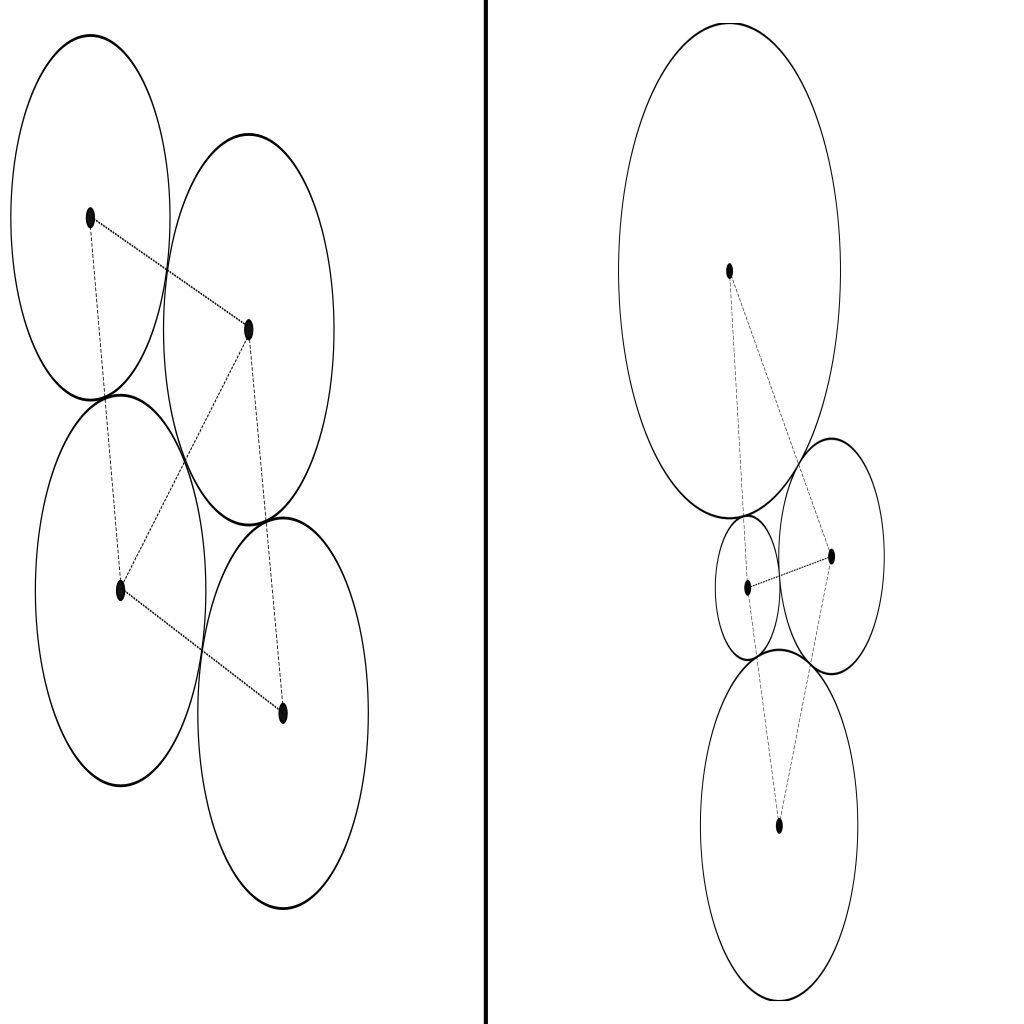
\includegraphics[width = 0.7\textwidth]{Chapter 4/12. 4 circle.png} \hspace{1 cm}
    \caption{Circle packing for the Laman graph on 4 nodes seen in Figure \ref{fig4: n = 4 Laman}. Left: drawn by hand. Right: generated using \texttt{circle\_packing}.} 
    \label{fig4: 4 node packing}
\end{figure}

\begin{figure}[htbp]
    \centering
    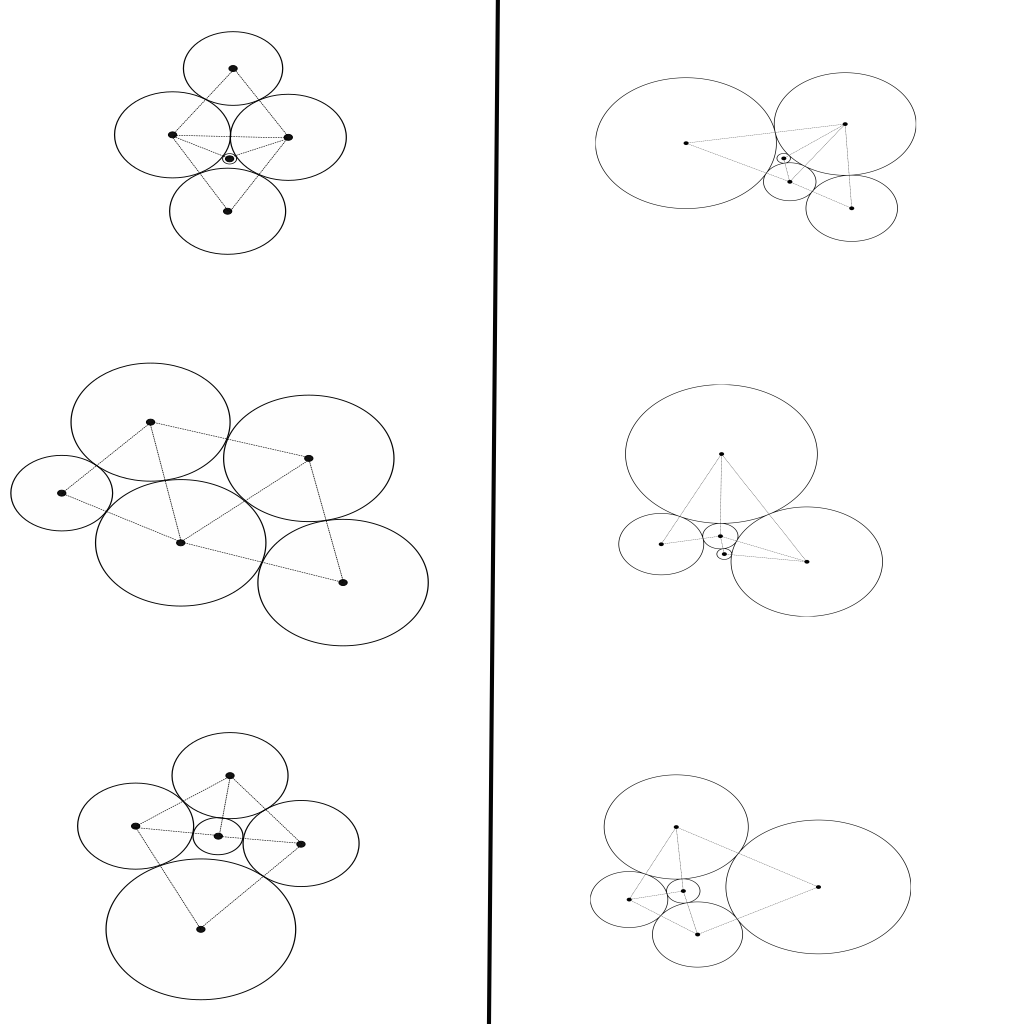
\includegraphics[width = 0.7\textwidth]{Chapter 4/13. 5 circle.png}
    \caption{Circle packings for the Laman graphs on 5 nodes seen in Figure \ref{fig4: n = 5 Laman}. Left column: drawn by hand. Right Column: generated using \texttt{circle\_packing}.}
    \label{fig4: 5 node packing}
\end{figure}

\begin{flushleft}
With these results, we confirm that the code developed in this module successfully finds a circle packing for a given planar graph.
\end{flushleft}

\section{Investigating the Conjecture}

\begin{flushleft}
To remind ourselves of what the conjecture is, we write it here once more:

\begin{center}
    \textit{``For every planar and minimally rigid graph, does there exist a circle packing that is also infinitesimally rigid?''}
\end{center}

Taking stock of everything we have;
\begin{itemize}
    \item Using \texttt{nauty}, we generated a list of non-isomorphic planar graphs with $n$ vertices and $2n-3$ edges.
    \vspace{-3mm}
    \item With the \texttt{Rigidity.py} module, we filter the list of planar graphs for minimally rigid ones with minimum degree 3.
    \vspace{-3mm}
    \item Using the \texttt{Circle\_Packing.py} module, we are able to generate the circle packing for a planar graph.
\end{itemize}

Therefore, our plan of attack will follow Algorithm 4.1.
\end{flushleft}
\begin{flushleft}
\textbf{Algorithm 4.1:} \footnote{use code language instead of plain english?}
\begin{enumerate}
    \item Generate a list of planar graphs on $n$ vertices using \texttt{nauty}.
    \vspace{-3mm}
    \item Use \texttt{find\_rigid\_graphs} from \texttt{Rigidity.py} and filter the list for minimally rigid planar graphs on $n$ vertices and minimum degree 3. Call this list \texttt{rigid\_graphs}.
    \vspace{-3mm}
    \item Initialize variables \texttt{attempt = 0}, \texttt{position = 0} and \texttt{max\_attempt = 500}.
    \vspace{-3mm}
    \item While \texttt{True}:
    \vspace{-3mm}
    \begin{enumerate}
        \item Increment \texttt{attempt} by 1.
        \vspace{-1mm}
        \item Call \texttt{circle\_packing} from \texttt{Circle\_Packing.py} for \texttt{rigid\_graphs[position]}.
        \vspace{-1mm}
        \item If the contact graph of the packing is isomorphic to \texttt{rigid\_graphs[position]} \textbf{\underline{and}} \texttt{check\_rigidity(contact\_graph)} returns \texttt{True} \textbf{\underline{and}} \texttt{position} is less than the length of \texttt{rigid\_graphs}:
        \begin{enumerate}
            \item Save \texttt{G}, \texttt{contact\_graph} \texttt{fig1}, \texttt{fig2} and \texttt{fig3}.
            \vspace{-1mm}
            \item Increment \texttt{position} by 1.
            \vspace{-1mm}
            \item Set \texttt{attempt} to 0.
        \end{enumerate}
        \vspace{-1mm}
        \item Else if the contact graph of the packing is isomorphic to \texttt{rigid\_graphs[position]} \textbf{\underline{and}} \texttt{check\_rigidity(contact\_graph)} returns \texttt{True} \textbf{\underline{and}} \texttt{position} is equal to the length of \texttt{rigid\_graphs}:
        \begin{enumerate}
            \item Save \texttt{G}, \texttt{contact\_graph} \texttt{fig1}, \texttt{fig2} and \texttt{fig3}.
            \vspace{-1mm}
            \item \texttt{break} out of the loop
        \end{enumerate}
        \vspace{-1mm}
        \item Else if the contact graph of the packing is not isomorphic to \texttt{rigid\_graphs[position]}, \textbf{\underline{or}} \texttt{check\_rigidity(contact\_graph)} returns \texttt{False}, \textbf{\underline{and}} \texttt{attempt} is equal to \texttt{max\_attempt}:
        \begin{enumerate}
            \item print ``Max attempts done, no viable packing found. Code terminating''
            \vspace{-1mm}
            \item \texttt{break} out of the loop
        \end{enumerate}
    \end{enumerate}
\end{enumerate}
\end{flushleft}

\begin{flushleft}
This algorithm is implemented in a script named \texttt{Rigid\_Packings.py}, and was used to verify whether all minimally rigid planar graphs on $n \in [3, \hdots, 10]$ have circle packings such that they are infinitesimally rigid. Therefore, it is possible to confirm that confirm that all minimally rigid planar graphs on $n \in [3, \hdots, 9]$ satisfy the conjecture. However, the code written here has displayed a few limitations, which we are going to address now.
\end{flushleft}

\subsection{Limitations to the code}

\subsubsection{1. Huge differences in radii}

\begin{flushleft}
When Algorithm 4.1 was implemented to one of the minimally rigid graphs on 9 nodes, the code failed to produce a circle packing after 500 attempts. Let this graph be known as $G$, and it is shown in Figure \ref{fig4: interesting}.
\end{flushleft}

\begin{figure}[htbp]
    \centering
    \begin{tabular}{c | c}
        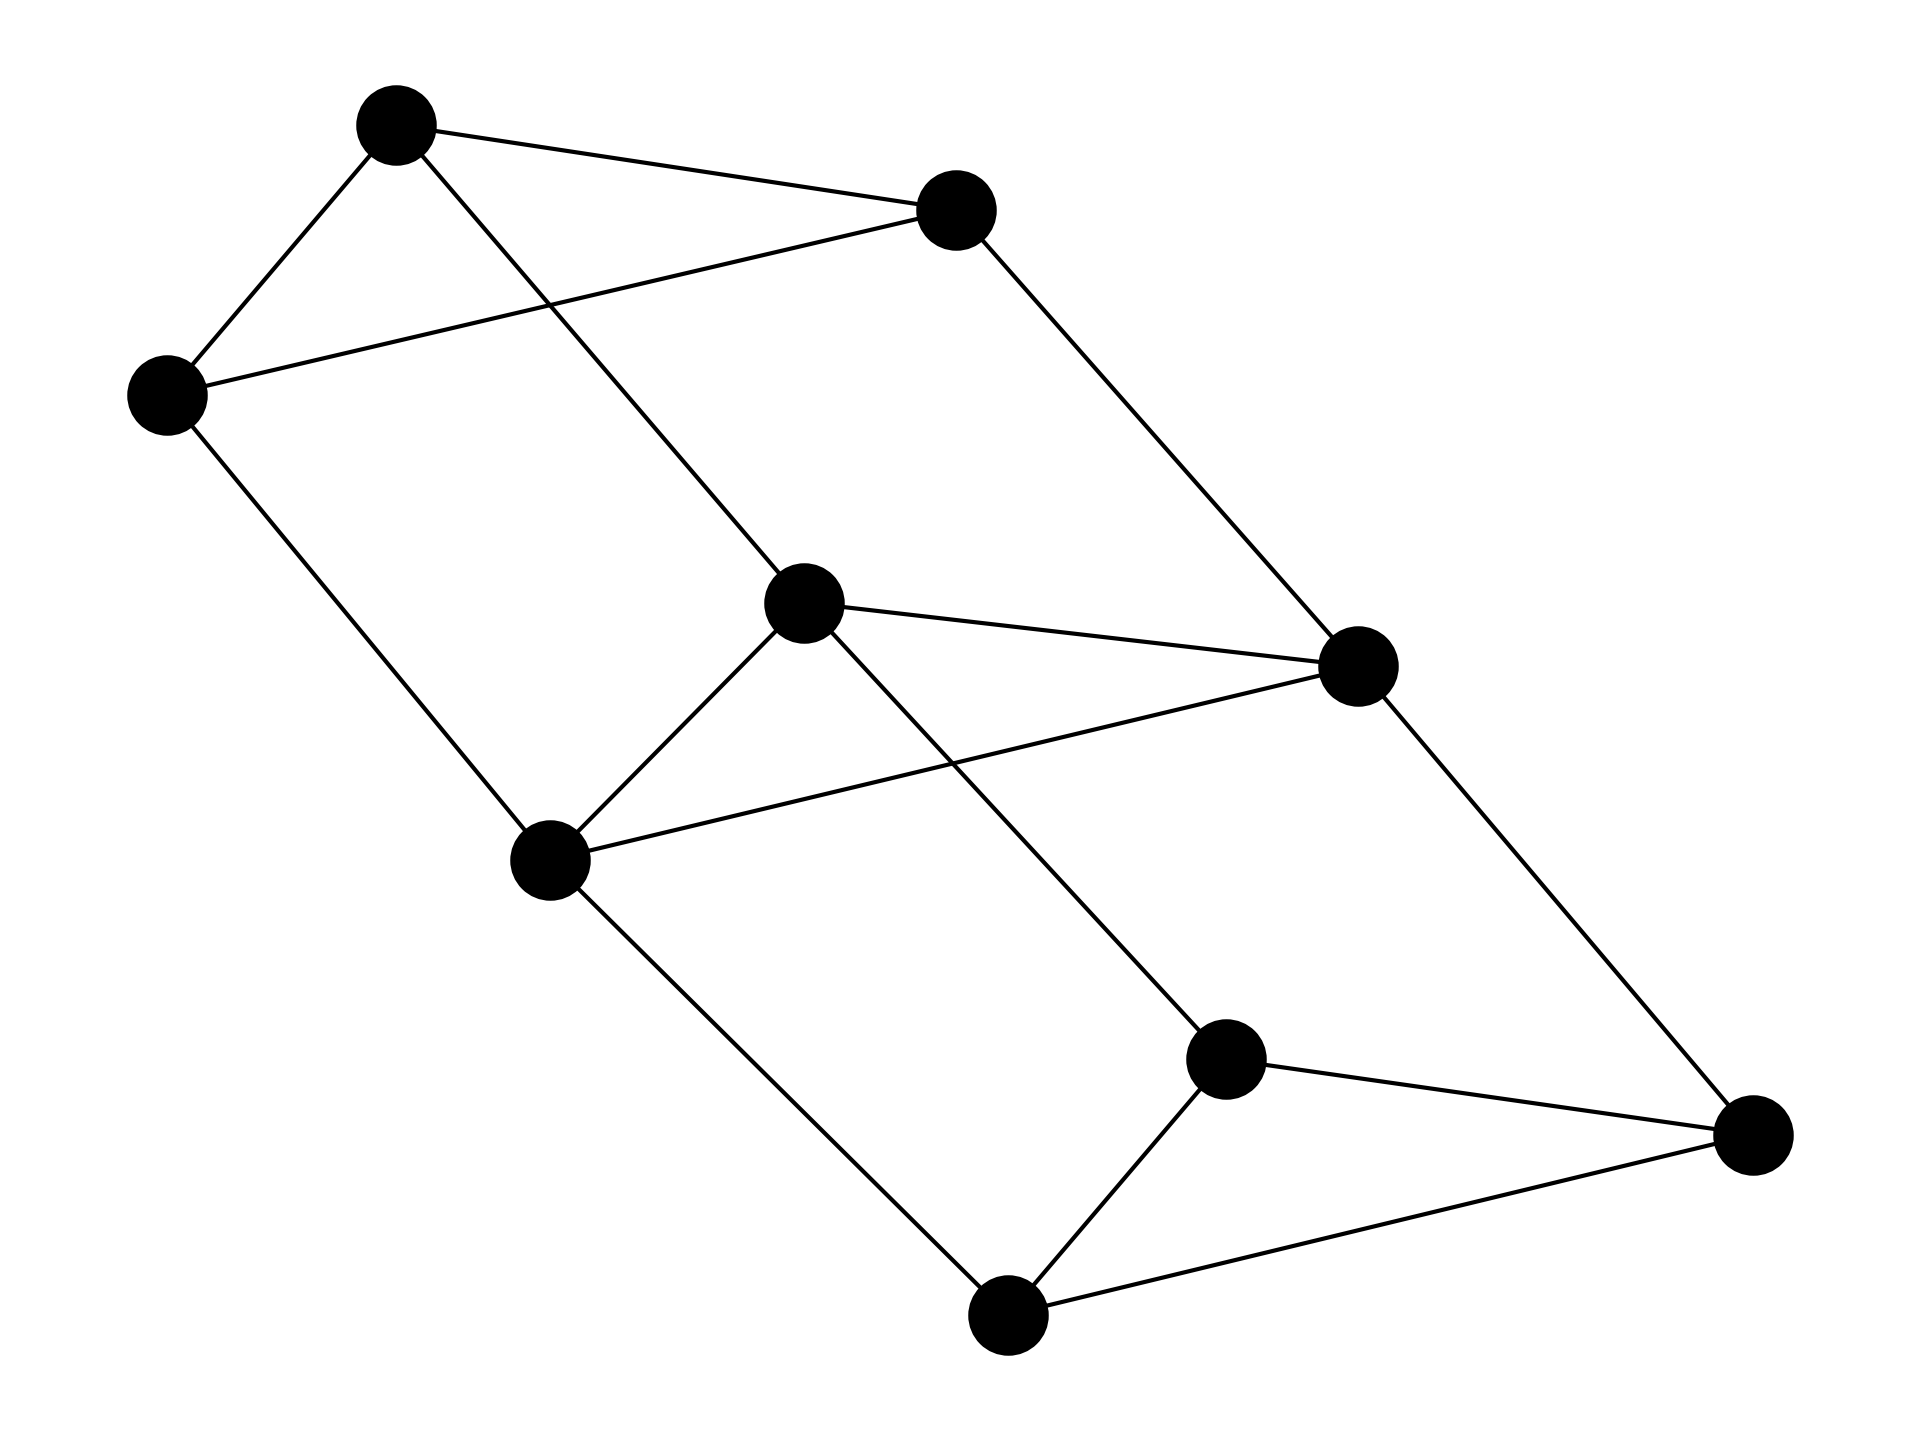
\includegraphics[width = 0.4\textwidth]{Chapter 4/14. interesting graph.png} & \hspace{5 mm} 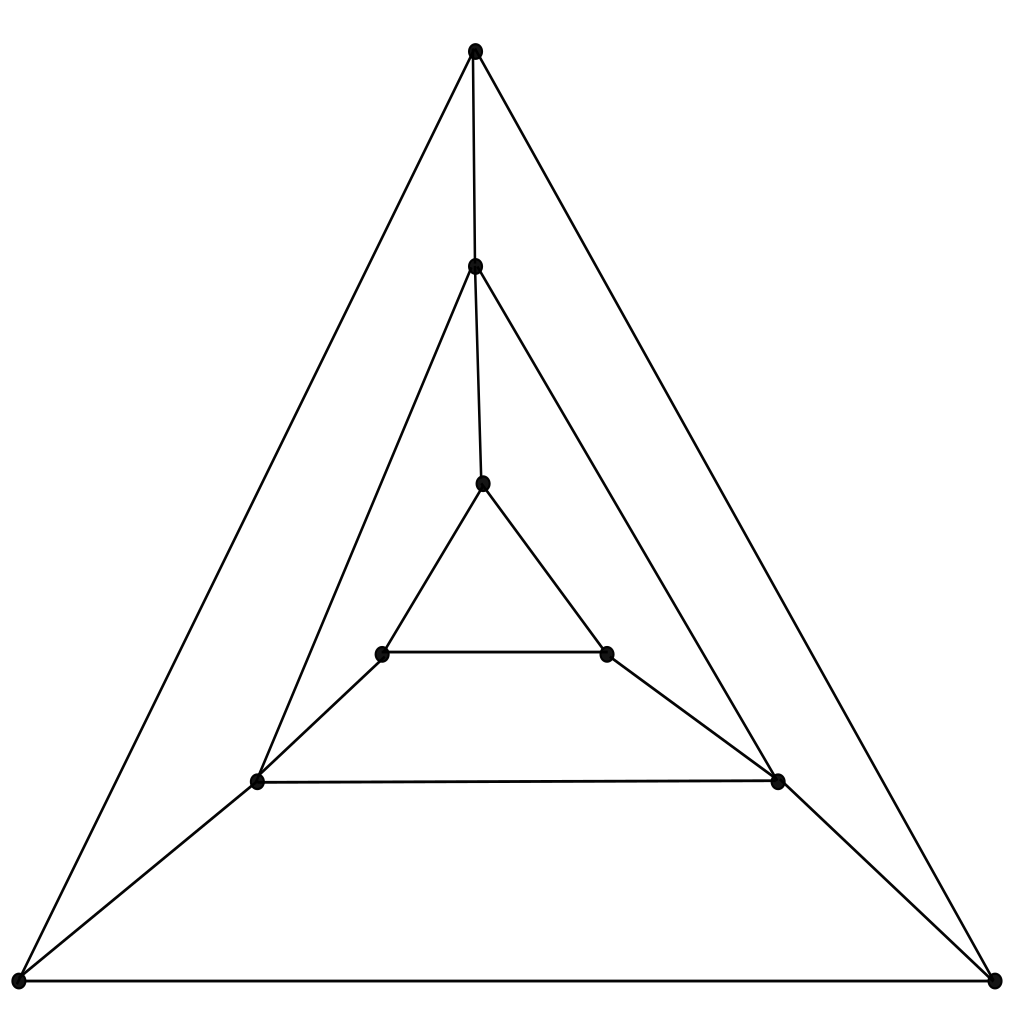
\includegraphics[width = 0.3\textwidth]{Chapter 4/15. interesting planar.png}   
    \end{tabular}
    \caption{Left: The graph $G$ that could not be packed computationally. Right: The planar vizualization of this graph}
    \label{fig4: interesting}
\end{figure}

\begin{flushleft}
Upon further investigation, it can be shown that this graph has a circle packing such that its contact graph is isomorphic to $G$. This is shown in Figure \ref{fig4: interesting packing}. As we can see, there is a vast difference between the radius of the largest circles on the `outside', and the inner-most circles. 
\end{flushleft}

\begin{figure}[htbp]
    \centering
    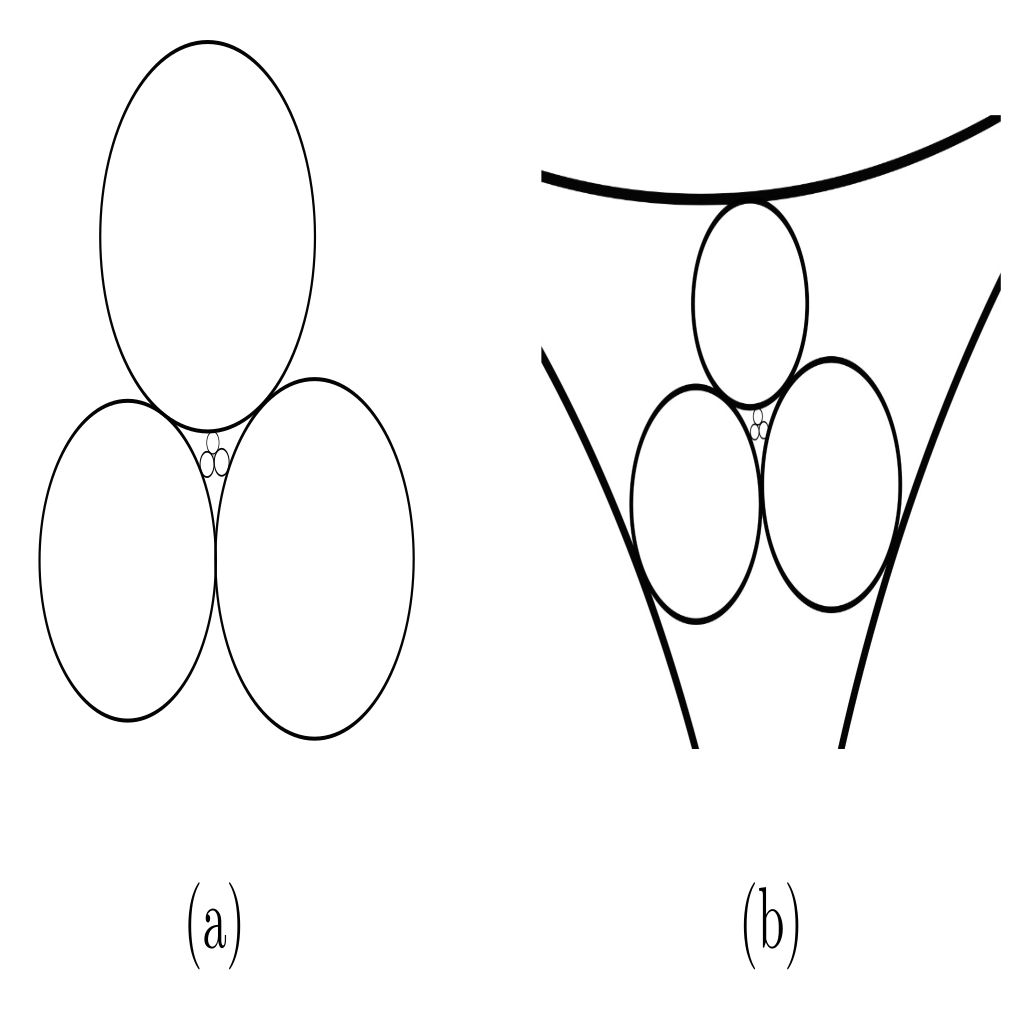
\includegraphics[width = 0.5\textwidth]{Chapter 4/16. interesting circle packing.png}
    \caption{(a) The circle packing for $G$. (b) The packing zoomed into the center to show the inner-most circles.}
    \label{fig4: interesting packing}
\end{figure}

\vspace{-5mm}
\begin{flushleft}
It is believed that due to this large difference in radii, the minimizer finds it difficult to place the circles correctly. This was tested by setting initial conditions in a configuration that matches the circle packing shown in Figure \ref{fig4: interesting packing}, but even then, the minimizer failed to provide the correct packing. 
\end{flushleft}

\begin{flushleft}
We can thereby conclude that even if an appropriate circle packing does exist for a graph, we may not be able to achieve it if the (absolute) difference between the biggest radius and the smallest radius in the packing is large. 
\end{flushleft}

\subsubsection{2. The initial conditions for increasing $n$}

\begin{flushleft}
The keen reader may have noticed that earlier, it was mentioned that Algorithm 4.1 was used to test minimally rigid graphs on $n \in [3, \hdots, 10]$ vertices, and that we can confirm the conjecture for $n \in [3, \hdots, 9]$ vertices. What about when $n = 10$?
\end{flushleft}

\begin{flushleft}
The issue here arises from the fact that we require packings isomorphic to the graph we start from. Suppose we start with a graph \texttt{G}. When \texttt{circle\_packing(G)} is called, it finds any possible circle packing satisfying the packing constraints. Later, in \texttt{Rigid\_Graphs.py}, \texttt{circle\_packing(G)} is called under a \texttt{while} loop. If the circle packing's contact graph is not isomorphic to \texttt{G}, then we restart the process and attempt to find a new packing with a new configuration of points and radii. 
\end{flushleft}

\begin{flushleft}
With 10 nodes to pack, the number of possible circle packings satisfying the packing constraints is quite substantial. Unless the initial configuration of points is sufficiently close to the solution we want, we will probably never attain it. Thus, the random generation of configurations is not an efficient method of creating suitable initial conditions as $n$ gets larger\footnote{mention that i tested random number of thousand graphs upto 10 attempts?}.
\end{flushleft}

\subsection{Tying It All Together}

\begin{flushleft}
With these results, we gain some understanding about the nature of the problem at hand. Although we know that a circle packing exists for a planar graph, trying to computationally show it and then verify its rigidity is a difficult task that we have made some progress towards here. Even with the limitations present, we can be somewhat confident about the truth of the problem we investigate as all the circle packings isomorphic to the graph it was derived from satisfies the conjecture. 
\end{flushleft}

\begin{flushleft}
(will need to flesh this out a little, work in progress)
\end{flushleft}